\documentclass[a4paper,11pt]{article}
\usepackage{algorithm, algorithmic}
\usepackage{color, graphics}
\usepackage{coling10}
\usepackage{times}
\usepackage{url}
\usepackage{latexsym}
\usepackage{amssymb}
\usepackage{epsfig}
\usepackage{amsmath}
\usepackage{amsfonts}
\usepackage{multirow}


%\setlength\titlebox{6.5cm}    % You can expand the title box if you
% really have to

\title{Relational Constraint-based Taxonomic Relation Identification}

\author{}

\date{}

\begin{document}
\maketitle

\newcommand{\ignore}[1]{}

\begin{abstract}
We present a novel approach to identifying relations between a pair of
concepts. We focus on identifying relations that are essential to
support textual inference: determining whether two concepts have an
ancestor relation, a sibling relation, or no relation. We develop a
machine learning-based approach that makes use of Wikipedia as a main
source for background knowledge, but we also propose an effective
approach of searching the Web to improve the coverage of our method
and support inference between concepts not present in Wikipedia. Our
key innovation is that, in order to accurately determine the relations
between concepts $C_1$ and $C_2$, we consider an automatically
generated collection of related concepts, evaluate all pairwise
relations, and use constraint-based inference to force them to cohere,
thus improving the local prediction of the pairwise relation
identification. We demonstrate that the inference technique
significantly enhances the local prediction methods and consequently
exhibit very large improvements over methods using existing knowledge
sources.

%%% Local Variables: 
%%% mode: latex
%%% TeX-master: "jupiter"
%%% End: 

\end{abstract}

\section{Introduction}
\ignore{Many data and knowledge management problems require some sort
  of textual inference. These range from query expansion and
  interpretation in information retrieval to query schema matching and
  question answering. \ignore{Especially, in advanced web search and
    contextual advertising, textual inference plays an important role
    as the core technique to finding related information that can
    attract users' interest. For instance, while searching for the
    reviews of {\em Nikon D90}, one may also be interested in reading
    the reviews for other {\em Nikon's cameras}, or {\em cameras} in
    general. To satisfy users' interest, advanced search engines need
    to be equipped with textual inference techniques that can perform
    search on related concepts in the index of web documents.}}

Structured knowledge bases like taxonomies and ontologies play
important roles in many computational linguistics tasks, such as
\cite{HSS03,673659}. Recently, the Textual Entailment challenge
~\cite{DaganGlMa06} has shown that taxonomic relations can greatly
help textual inference which requires the use of large amounts of
background knowledge. For example, it may be important to know that a
{\em blue Toyota} is neither a {\em red Toyota} nor a {\em blue
  Honda}, but that all are cars, and even Japanese cars. Work in
Textual Entailment has argued quite convincingly,
(e.g.~\cite{maccartney-manning:2008:PAPERS}), that many inferences are
largely compositional and depend on the ability of models to recognize
taxonomic relations between noun phrases.

In this paper, we focus on identifying two general types of taxonomic
relations - {\em ancestor} and {\em sibling}. An ancestor relation and
its directionality can help us deduce that a statement with respect to
the child (e.g. {\em cannabis}) holds for an ancestor (e.g. {\em
  drugs}) as in the following example, taken from the textual
entailment challenge dataset:

{\small
  \begin{quote}
    {\bf T}: Nigeria's NDLEA has seized 80 metric tonnes of {\em
      cannabis} in one of its largest ever hauls, officials say.

    {\bf H}: Nigeria seizes 80 tonnes of {\em drugs}.
  \end{quote}
}

Similarly, it is important to know of a sibling relation to infer that
a statement about {\em Taiwan} may (without additional information)
contradict an similar statement with respect to {\em Japan} since
these are different countries, as in the following:

{\small
  \begin{quote}

    {\bf T}: A strong earthquake struck off the southern tip of {\em
      Taiwan} at 12:26 UTC, triggering a warning from Japan's
    Meteorological Agency that a 3.3 foot tsunami could be heading
    towards Basco, in the Philippines.

    {\bf H}: An earthquake strikes {\em Japan}.
  \end{quote}
}

Several work has been devoted to acquiring structured taxonomies and
ontologies resulting in structured knowledge bases such as the {\em
  augmented WordNet} \cite{Snow2006} and \textsc{Yago}
\cite{suchanek2007WWW}, which represent taxonomic information of
individual concepts. We believe that these acquired structured
knowledge bases are important resources to support classification of
taxonomic relations. However, these resources usually suffer from
noise and, especially, uncertainty with respect to each concept,
making it difficult to support robust classification of taxonomic
relations between two given concepts.

\ignore{A lot of work has been devoted to acquiring semantic taxonomies and
ontologies \cite{Snow2006,wikitaxo07,suchanek2007WWW} resulting in
structured knowledge bases such as {\em augmented WordNet} and
\textsc{Yago} which represent taxonomic information about individual
concepts (See Sec.~\ref{sec:related-work}). However, as we show, these
suffer from limited coverage and, more importantly, need to represent
uncertainty with respect to each concept, making it difficult to
support robust classification of taxonomic relations between two given
concepts.}

% In this paper, we present a novel approach to the fundamental
% problem of recognizing taxonomic relations between two given
% concepts.

\ignore{Identifying and classifying taxonomic relations between two
  given concepts serves a different purpose and is distinct from that
  of Open Information Extraction \cite{BCSBE07}, On-Demand Information
  Extraction \cite{Sekine06} and other effort to recognize {\em easy
    to find} facts in a given
  corpus~~\cite{davidov-rappoport:2008:ACLMain2,pacsca-vandurme:2008:ACLMain}--capitalizing
  on local co-occurrence of concepts to generate databases of
  open-ended facts. It is also different from the supervised relation
  extraction~\cite{RothYi04} effort which requires additional
  supervised data to learn new relations.}

%
%
% The key reason is that the knowledge acquisition methods alluded to
% know of {\em X} and {\em Y} only if they have occurred in an
% explicit way and in close proximity in a sentence.  Indeed, we know
% of no successful application of the large scale existential
% knowledge acquisition efforts to textual inference.



\ignore{There is a need to fuse information from multiple sources,
  including unstructured text (e.g., the web) in order to determine
  the taxonomic relation between a pair of concepts.}

\ignore{ This paper proposes to address the problem of on-the-fly
  taxonomic relation identification and classification in a form that
  is directly applicable to textual inference. In the paper of
  \cite{maccartney-manning:2008:PAPERS}, it is shown that taxonomic
  relations are key relations for textual inference. In their work,
  {\em sibling} relation is referred as {\em alternation}, and {\em
    ancestor} (or {\em is-a}) relation is referred as {\em forward
    entailment} and {\em backward entailment}. Following their
  argument, we expect that the resource developed in this work can be
  used compositionally to support robust textual inference.  }
\ignore{Specifically, our system accepts two input concepts as
  arguments (these could be entities or noun phrases) and identifies
  the relation between them \ignore{along with its possible
    label}. For example, we identify that {\em global warming} and
  {\em food crisis} are in a {\em sibling} relation, and the concept
  of {\em economic problems} is in an {\em ancestor} relation with
  both of them. We focus here on the {\em ancestor} (or {\em is-a})
  relation and the {\em sibling} relation that were identified as key
  relations also in \cite{maccartney-manning:2008:PAPERS} (they call a
  {\em sibling} relation an {\em alternation}, and our {\em ancestor}
  relation {\em forward entailment} and {\em backward
    entailment}). Following their argument, we expect that the
  resource developed in this work can be used compositionally to
  support robust textual inference.}

\ignore{ Our approach can discover whether two input entities pose an
  alternation (or non-exhaustive exclusion) relation ({\em red} $|$
  {\em green}), forward entailment ({\em Mel Gibson} $\sqsubset$ {\em
    actor}), reverse entailment ({\em flower} $\sqsupset$ {\em lily}),
  or independence ({\em Boeing 747} $\#$ {\em Valentine}). }

In this paper, we present our system to identify taxonomic relations
using machine learning-based approach. More importantly, we describe
our constraint-based inference model that incorporates relational
constraints as prior knowledge to accurately identify taxonomic
relations. Furthermore, we present a novel approach to leveraging an
existing knowledge base, which is by itself weaker than our system in
identifying taxonomic relations, to provide useful information to our
inference model.

\ignore{Constrained optimization-based decision algorithm to construct
  an effective taxonomic relation classifier. We show that our
  approach significantly improves taxonomic relation identification
  relative to existing structured knowledge sources.}

\ignore{Our key technical contribution is a constraint-based framework
  that makes use of relational constraints in a global inference
  process that accurately identifies taxonomic relations. Our
  inference algorithm makes use of an accurate classifier we develop,
  which returns, for a given pair of concepts, a distribution over
  possible taxonomic relations; this classifier is applied multiple
  times, on an automatically generated network of concepts that are
  related to the target pair, and the constrained optimization
  technique is used to force these decisions to cohere across the
  network. This results in improving the accuracy of each of the
  predicted relations in the network.}
%
\ignore{Our basic classifier makes use of Wikipedia and its category
  structure. On one hand, this guarantees growing coverage but, on the
  other, necessitates taking into account the non-uniformity and level
  of noise in this resource.  Our algorithmic approach therefore
  treats Wikipedia and its category structure as an open resource and
  uses statistical text mining techniques to gather robust
  information. And, while Wikipedia has broad coverage, there is a
  need to go beyond it.  We suggest a simple but efficient technique
  to accomplish this using web search, and show its effectiveness when
  at least one of the target concepts is not mentioned in Wikipedia.}

%
\ignore{For example, the concept {\em Ford} appears many times in
  Wikipedia and is part of a large number of categories. As a {\em
    president}, mentions of {\em Ford} are consistent with mentions of
  other presidents. However, {\em Ford} also appears in other senses,
  for example, related to the {\em car} industry.  We need to
  disambiguate it, determine which category it belongs to and, within
  this category, which specific concept is intended. In order to
  disambiguate it, we make use of the context provided by the concept
  pair---{\em Ford} in ({\em Ford}, {\em Nixon}) is probably different
  than the one in ({\em Ford}, {\em Chevrolet}) as well as the one in
  ({\em Ford}, {\em Iacocca}).}
%
\ignore{Textual inference is driven by background
  knowledge. Therefore, the notion of {\em prominence} is
  essential. Most people know that {\em Michael Jordan} is a former
  NBA player, but they most likely do not know the {\em Michael
    Jordan} who attends school with the authors.  Consequently, unless
  additional knowledge is given, a textual inference system should
  assume that {\em Michael Jordan} is a basketball player. This is why
  we use Wikipedia as our background knowledge source. Moreover, under
  the assumption that in textual inference applications we are in
  search of some notion of ``common sense'' knowledge, we make use of
  a notion of prominence with respect to a given text collection (in
  this case, with respect to Wikipedia itself).}
  %


\ignore{Our key technical contribution is a novel approach that makes
  use of constraint-based inference with relational constraints to
  accurately identify relations; we make use of our machine learning
  approach multiple times, on automatically generated network of
  concepts that are related to the target pair, and use constrained
  optimization techniques to force these decisions to be coherent,
  thus improving the accuracy of the decision.}

\ignore{We measure the performance of our system over a large number
  of pairs chosen from over 40 semantic classes. We compare it with
  other large scale efforts to identify relations between
  concepts. For example we show that, even when all concepts are
  covered by the {\em extended WordNet}~\cite{Snow2006}, our system
  still significantly outperforms that system. }
%
% We also show examples indicating the contribution of our relation
% identification to textual inference.

\ignore{ In summary, the contributions of this paper are:

  \begin{enumerate}
    % \item The definition of a taxonomic relation identification
    %   problem so that it is directly relevant to supporting textual
    %   inference
  \item The development of a robust and accurate machine
    learning-based approach to classify taxonomic relations.
  \item A constraint-based inference model that leverages relational
    constraints as prior knowledge to accurately identify taxonomic
    relations.
  \item An approach to make use of an existing knowledge base, which
    by itself is weaker than our relation identifier, to provide
    useful information to the inference process.
  \end{enumerate}
}

\ignore{ In an extensive experimental study we show that our approach
  significantly improves taxonomic relation identification relative to
  existing structured knowledge sources.}

The rest of this paper is organized as follows:
Sec. \ref{sec:overview-algorithm} gives an overview of our approach.
We then present our learning component in Sec. \ref{sec:learning}.
Sec. \ref{sec:inference} describes our inference model that leverages
global relational constraints to infer taxonomic
relations. Sec. \ref{sec:experiments} presents our experimental study,
and Sec. \ref{sec:related-work} describes related work.

\ignore{In Sec. \ref{sec:inference} we present the constraint-based
  inference model that makes used of global relational constraints to
  infer concepts' taxonomic relations. As shown, in order to generate
  a network of related concepts for the inference process we leverage
  the \textsc{Yago} ontology. Our machine learning-based component is
  used to make local prediction on taxonomic relations and is
  described in Sec. \ref{sec:learning}. Sec. \ref{sec:experiments}
  presents our experimental evaluation, and
  Sec. \ref{sec:related-work} describes some of the related work.}
% We conclude the paper in Sec. \ref{sec:conclusions}.

 \ignore{Notably, our algorithmic approach is trained with a small
  number of annotated examples and generalizes well across semantic
  classes.}

\ignore{The rest of this paper is organized as follows. In
  Section~\ref{sec:relatedwork}, we briefly mention about previous
  work that inspired our approach.  Section~\ref{sec:approach}
  formalizes the problem and describes our algorithmic approach to
  relation detection and classification. Our experiments and results
  are described in Section \ref{sec:experiments}. Discussion and
  future work are in Section \ref{sec:discussion}.}


%%% Local Variables:
%%% mode: latex
%%% TeX-master: "jupiter"
%%% End:


\section{Taxonomic Relation Identification: An Overview}
\label{sec:overview-algorithm}
In this section, we present our overall algorithm addressing
the problem of identifying taxonomic relation of concepts.

Inputs of our algorithm are a pair of target concepts ($X$, $Y$) and a
trained taxonomic relation classifier $\mathcal{R}$, which is used to
provide a distribution of confidences over all possible taxonomic
relations between any two concepts. The algorithm's output is the
taxonomic relation of $X$ and $Y$, which can be (1) $X$ is an {\em
  ancestor} of $Y$, denoted by $X \leftarrow Y$; (2) $X$ is a {\em
  child} of $Y$, denoted by $X \rightarrow Y$; (3) $X$ and $Y$ are
{\em siblings}, denoted by $X \leftrightarrow Y$; or (4) $X$ and $Y$
have {\em no relation}, denoted by $X \nleftrightarrow Y$.

%%%%%%%%%%%%%%%%%%%%%%%%%%%%%%%%%%%%

\ignore{Input of our problem is a pair of concepts ($X$, $Y$), and output is
their taxonomic relation which can be (1) $X$ is an {\em ancestor} of
$Y$, denoted by $X \leftarrow Y$; (2) $X$ is a {\em child} of $Y$,
denoted by $X \rightarrow Y$; (3) $X$ and $Y$ are {\em siblings},
denoted by $X \leftrightarrow Y$; or (4) $X$ and $Y$ have {\em no
  relation}, denoted by $X \nleftrightarrow Y$.}

\ignore{
\begin{enumerate}
\item $X$ is an ancestor of $Y$, denoted by $X \leftarrow Y$.
\item $X$ is a child of $Y$, denoted by $X \rightarrow Y$.
\item $X$ and $Y$ are siblings, denoted by $X \leftrightarrow Y$.
\item $X$ and $Y$ have no relation, denoted by $X \nleftrightarrow Y$.
\end{enumerate}
}

\ignore{ Our approach consists of two key components: (1) a machine
  learning-based algorithm to classify taxonomic relations; and (2) a
  constraint-based inference model to make final decision using
  relational constraints of taxonomic relations.  }

\ignore{
\begin{enumerate}
\item A machine learning-based algorithm to classify concept relations.
\item A constraint-based inference model to make final decision using
  relational constraints enforced among concept relations.
\end{enumerate}
}

Figure \ref{fig:rel-know-iden-alg} presents our overall algorithm to
identify taxonomic relation of $X$ and $Y$. The algorithm consists of
two main components (1) a machine learning-based algorithm to learn a
local taxonomic relation classifier; and (2) a constraint-based
inference model that makes use of related concepts extracted for $X$
and $Y$ to make final decision on taxonomic relation of X and Y.  Both
components use the same Wikipedia index as a knowledge source to
extract features of input concepts and related concepts to learn the
local classifier and do inference as well.

The identification component (B) makes prediction on the taxonomic
relation between $X$ and $Y$ using $\mathcal{R}$ as its local
classifier.  Given two concepts $X$, and $Y$, function
\texttt{isNotWikipediaConcept} determines if they are {\em Wikipedia
  concepts} or {\em non-Wikipedia concepts} by searching the concept
space in Wikipedia. If a concept is {\em non-Wikipedia} (i.e. it does
not have a Wikipedia page), the algorithm tries to find a replacement
for it by performing a web search via function
\texttt{findReplacement}. Replacing concepts are expected to be {\em
  Wikipedia concepts} and in the same semantic class with the input
concepts. After that, function \texttt{extractRelatedConcepts} returns
list $\mathcal{Z}$ of additional concepts which are related to $X$ and
$Y$. The algorithm passes the two input concepts, local classifier
$\mathcal{R}$ and list $\mathcal{Z}$ to function \texttt{doInference},
which solves a constraint-based optimization problem and returns
$\ell^*$, the taxonomic relation of $X$ and $Y$.

\ignore{We then use two input concepts (or their
  replacements) to build a list of Wikipedia articles that represents
  each input. Following, a machine learning-based classifier is used
  to identify the taxonomic relations between two concepts. Finally,
  we make a final decision using an inference model within a
  constraint-based framework that explores relational constraints
  enforced among concepts involved.}

\begin{figure}[!t]
  \begin{centering}
    {\scriptsize
      \fbox{
        \begin{minipage}{6in} 
          \begin{tabbing}
            {\textsc{A. Learning local classifier $\mathcal{R}$}~~~~~~~~~~~~~~~~~}\\
            \qquad {\textsc{Input}}: ~~~Training set  \\
            \qquad \qquad \qquad \qquad $\mathcal{D}$ = \{taxonomic-relation-annotated concept pairs\} \\
            \qquad \qquad \qquad Wikipedia index $\mathcal{W}$ \\
            \qquad {\textsc{Output}}: A local taxonomic relation classifier $\mathcal{R}$ \\
            \\
            \qquad 1. ~~~~$\mathcal{R} \leftarrow$ \texttt{train($\mathcal{D}$, $\mathcal{W}$)} \\
            \\
            {\textsc{B. On-the-fly Taxonomic Relation Identification}~~~~~~~~~~~~~~~~~~~~~~}\\
            \qquad {\textsc{Input}}: ~~~A concept pair ($X$, $Y$) \\
            \qquad \qquad \qquad A trained taxonomic relation classifier \\
            \qquad \qquad \qquad \qquad $\mathcal{R}$ used to make local prediction. \\
            \qquad \qquad \qquad Wikipedia index $\mathcal{W}$ \\
            \qquad {\textsc{Output}}: Taxonomic relation $\ell^*$ of $X$ and $Y$ \\
            \\
            \qquad 1. ~~~~If \texttt{isNotWikipediaConcept($X$,  $\mathcal{W}$)}, then \\
            \qquad \qquad \qquad $X \leftarrow \texttt{findReplacement}(X, Y)$ \\
            %\qquad End if \\
            \qquad \qquad If \texttt{isNotWikipediaConcept($X$,  $\mathcal{W}$)}, then \\
            \qquad \qquad \qquad $Y \leftarrow \texttt{findReplacement}(Y, X)$ \\
            %\qquad End if \\
            \\     
            \qquad 2. ~~~$\mathcal{Z} \leftarrow \texttt{extractRelatedConcepts}(X,Y)$ \\
            \\
            \qquad 3. ~~~$\ell^* = \texttt{doInference}(X,Y,\mathcal{Z},\mathcal{R},\mathcal{W})$ \\
            \\
            \qquad \textsc{Return}: $\ell^*$; \\
          \end{tabbing}
        \end{minipage}
      }
  }
\end{centering}
\caption{On-the-fly taxonomic relation identification algorithm.}
\label{fig:rel-know-iden-alg}
\end{figure}

\ignore{
\begin{figure}[!t]
  \begin{centering}
    {\scriptsize
      \fbox{
        \begin{minipage}{6in} 
          \begin{tabbing}
            {\textsc{On-the-fly Taxonomic Relation Identification}~~~~~~~~~~~~~~~~~~~~~~~~~~~~}\\
            \qquad {\textsc{Input}}: A concept pair ($X$, $Y$) \\
            \qquad {\textsc{Output}}: Relation of $X$ and $Y$ \\
            \\
            \qquad If $X$ is a {\em non-Wikipedia concept} then \\
            \qquad \qquad $X \leftarrow \texttt{findReplacement}(X, Y)$ \\
            %\qquad End if \\
            \qquad If $Y$ is a {\em non-Wikipedia concept} then \\
            \qquad \qquad $Y \leftarrow \texttt{findReplacement}(Y, X)$ \\
            %\qquad End if \\
            \\     
            \qquad Building Wikipedia-article representation $F(X)$ and $F(Y)$ \\
            \qquad $R = \texttt{classifyTaxonomicRelation}(F(X),F(Y))$ \\
            \qquad $R^* = \texttt{inference}(X,Y,R)$ \\
            \\
            \qquad \textsc{Return}: $R^*$; \\
          \end{tabbing}
        \end{minipage}
      }
  }
\end{centering}
\caption{On-the-fly taxonomic relation identification algorithm.}
\label{fig:rel-know-iden-alg}
\end{figure}
}


\ignore{In our work, we use Wikipedia as the main source of background
  knowledge used to recognize concept relations.}

Functions \texttt{extractRelatedConcepts} and \texttt{doInference} are
described in details in Sec. \ref{sec:inference}.

The learning component (A) trains a local classifier $\mathcal{R}$ for
the taxonomic relation identification, and is described in Sec. \ref{sec:learning}.

Although most commonly used concepts can be found in Wikipedia, there
is still a need to cover the {\em non-Wikipedia concepts} to improve
the coverage of the algorithm. Briefly, function
\texttt{findReplacement}($X$, $Y$) takes a {\em non-Wikipedia concept}
$X$ and a supporting concept $Y$ as its input. The function searches
the web to find a {\em Wikipedia concept} $X'$ which is in the same
semantic class of $X$ to be its replacement. Our method was motivated
by \cite{1321585}.  In our work, we use the Yahoo! Web Search
APIs\footnote{http://developer.yahoo.com/search/web/} to search for
list structures in web documents such as ``... $\left < delimiter
\right >$ c$_a$ $\left < delimiter \right >$ c$_b$ $\left < delimiter
\right >$ c$_c$ $\left < delimiter \right >$ ...'' ($X$ and $Y$ are
among c$_a$, c$_b$, c$_c$, ...). For text snippets that contain the
patterns of interest, we extract $c_a$, $c_b$, etc. as replacement
candidates. To reduce noise, we constrain the list structure to
contain at least 4 concepts that are no longer than 20 characters
each. The candidates are ranked based on their occurrence
frequency. The top candidate in the Wikipedia concept space is used as
replacement.

%%% Local Variables: 
%%% mode: latex
%%% TeX-master: "jupiter"
%%% End: 


\section{Learning Taxonomic Relations}
\label{sec:learning}
\ignore{ Given two input concepts ($X$, $Y$), we first disambiguate
  them to get lists of relevant Wikipedia articles. We then extract
  features of disambiguated concepts and train a supervised
  multi-class classifier to classify relations between them.  }

In this section, we describe our machine learning-based classifier for
taxonomic relations of concepts. For each input concept in the input
pair, we first build its article representation by searching for a
list of relevant articles in Wikipedia. To do this, we first use both
concepts to search the Wikipedia index, and then extract important
keywords in the titles and categories of the returned articles. The
extracted keywords are combine with each input concept to create a
final query that is used to search for a list of relevant articles in
Wikipedia. From now on, we use {\em the titles of $X$}, {\em the texts
  of $X$}, and {\em the categories of $X$} to refer to the titles,
texts, and categories of the associated articles of concept $X$. As a
learning algorithm, we use a regularized averaged Perceptron
\cite{FreundSc99}. Below are features extracted for pair ($X$,$Y$)
using their lists of relevant articles.

\ignore{
\begin{table*}[!t]
  \tiny
  \centering
  \begin{tabular}{|p{0.5in}|p{3.7in}|p{1.6in}|}
    \hline
    {\bf Concept/Title} & {\bf Text} & {\bf Categories} \\
    \hline
    \hline
    President of the United States & \textit{The President of the United States is the head of state and head of government of the United States and is the highest political official in the United States by influence and recognition. The President leads the executive branch of the federal government and is one of only two elected members of the executive branch...} & \textit{Presidents of the United States, Presidency of the United States} \\
    \hline
    George W. Bush & \textit{George Walker Bush; born July 6, 1946) served as the 43rd President of the United States from 2001 to 2009. He was the 46th Governor of Texas from 1995 to 2000 before being sworn in as President on January 20, 2001...} & \textit{Children of Presidents of the United States, Governors of Texas, Presidents of the United States, Texas Republicans...} \\
    \hline
    Gerald Ford & \textit{Gerald Rudolff Ford (born Leslie Lynch King, Jr.) (July 14, 1913 – December 26, 2006) was the 38th President of the United States, serving from 1974 to 1977, and the 40th Vice President of the United States serving from 1973 to 1974.} & \textit{Presidents of the United States, Vice Presidents of the United States, Republican Party (United States) presidential nominees...} \\
    \hline
  \end{tabular}
  \caption{Examples of texts and categories of the concepts from Wikipedia: {\em President of the United States}, {\em George W. Bush} and {\em Gerald Ford}.}
  \label{tab:snippets}
\end{table*}
}

\ignore{
  \subsection{Concept Disambiguation}
  \label{sec:conc-disamb}

  \ignore{In this paper, we address the problem of identifying
    relation between concepts.  Our problem is different than other
    previous work on relation extraction. Most of traditional relation
    extraction tasks often focus on extracting all possible entity
    pairs that follow some pre-defined relations (e.g. LocatedIn,
    BornInYear, AuthorOf, etc.) in big corpora
    \cite{banko-etzioni:2008:ACLMain}. Some other previous work
    extracting all possible entity pairs and relations from big
    corpora with a list of same class entities as the start point
    \cite{davidov-rappoport:2008:ACLMain2}. Another direction of
    relation extraction is to extract all possible instances of a
    given class, or in the same class of given instances
    \cite{WangCohen09,kozareva-riloff-hovy:2008:ACLMain}.}

  \ignore{In this paper, we limit the relations of interest to
    \emph{Ancestor}, \emph{Sibling}, or \emph{None} relations.}

  Given two input concepts ($X$, $Y$), we must first disambiguate
  them. The more accurate the disambiguation is, the more precise the
  relation recognition is. For example, the concept \emph{Ford} in the
  concept pair \emph{(Bush, Ford)} may refer to several concepts, such
  as \emph{Ford Motor Company}, president \emph{Gerald Ford}, or
  \emph{Ford, Wisconsin - USA}. Our approach is motivated by observing
  that the concept \emph{Bush} can be used to disambiguate \emph{Ford}
  and vice versa. Ultimately, we can place articles about \emph{George
    W. Bush} and \emph{Gerald Ford} the top of a retrieved articles
  list for the two input concepts \emph{Bush} and \emph{Ford}.

  Figure \ref{fig:entity-disamb} shows the concept disambiguation
  algorithm.

  \begin{figure}[!t]
    \begin{centering}
      {\scriptsize \fbox{
        \begin{minipage}{6in} 
          \begin{tabbing}
            {\textsc{Concept Disambiguation Algorithm}} \\
            \qquad {\textsc{Input}}: Concept pair ($X$, $Y$); Number of top tokens $N$ ~~~~~~~ \\
            \qquad {\textsc{Output}}: Two list of relevant articles for $X$ and $Y$. \\
            \\
            \qquad Query $q \leftarrow $ Concatenating $X$ and $Y$; \\
            \qquad $\mathcal{L} = \texttt{ESA}(q)$; \\ %// return a list of relevant articles to $X$ and $Y$ \\
            \qquad $\mathcal{C} = \texttt{getCategories}(\mathcal{L})$; \\
            \qquad $\mathcal{T} = \texttt{tokenize}(\mathcal{C})$; \\
            \qquad $\mathcal{T}_{top} = \texttt{topTfidf}(\mathcal{T}, N)$; \\ %// pick top $N$ tokens\\
            \\
            \qquad Query $q_X \leftarrow $ Concatenating $X$ and tokens in $\mathcal{T}_{top}$; \\
            \qquad Query $q_Y \leftarrow $ Concatenating $Y$ and tokens in $\mathcal{T}_{top}$; \\
            \qquad $\mathcal{A}_X = \texttt{search}(q_X)$; \\
            \qquad $\mathcal{A}_Y = \texttt{search}(q_Y)$; \\
            \\
            \qquad \textsc{Return}: $\mathcal{A}_X$ and $\mathcal{A}_Y$; \\
          \end{tabbing}
        \end{minipage}
      } }
  \end{centering}
  \caption{Concept disambiguation algorithm. The algorithm takes two
    input concepts, disambiguates them and returns a list of relevant
    Wikipedia articles for each.}
  \label{fig:entity-disamb}
  \end{figure}

  Function \texttt{ESA}({\em query}) retrieves the most semantically
  relevant articles in Wikipedia to {\em query}.  We use Explicit
  Semantic Analysis (ESA) \cite{GabrilovichMa07} to retrieve
  semantically relevant articles in Wikipedia for two given
  concepts. For all articles in the relevant list, we extract and keep
  their categories by the function \texttt{getCategories}({\em
    list}). All categories are then tokenized and weighted using the
  TF-IDF score. Only top $N$ tokens, which are different from the two
  input concepts, are considered. Each input concept is then
  concatenated with the top weighted tokens to create a new query
  that, in turn, is the input for the \texttt{search}({\em query})
  function. Our search function returns relevant articles in Wikipedia
  for the input {\em query}. The lists of relevant articles are later
  used to provide features for the local relation classifier. If a
  returned list is empty, its corresponding concept is considered as a
  {\em non-Wikipedia concept}.  }


%\subsection{Learning Relations}
%\label{sec:learner}

\ignore{ We first extract expressive features associated with the two
  input concept pairs. These features are necessarily independent of
  the semantic class of the given concepts so that our classifier can
  generalize well. Recall that, after concept disambiguation, each
  input concept is associated with a list of relevant articles in
  Wikipedia. In other words, from these articles, an input concept is
  represented with several Wikipedia titles, texts, and categories.
  From now on, we use {\em the titles of concept $X$} to refer to the
  titles of the articles associated with concept $X$; similarly for
  {\em the texts of concept $X$}, and {\em the categories of concept
    $X$}. As a learning algorithm, we use a regularized averaged
  Perceptron \cite{FreundSc99}.  }

\ignore{The features selected for our learning problem include the
  words used in the associated articles, the association information
  between two concepts, and the overlap ratios of important
  information between the concepts and the articles. We describe these
  features below.}

%\subsubsection{Bags of Words}

\ignore{{\bf Bags of words}: One of the most important features in
  recognizing relations between concepts are the words used in
  associated articles. An article in Wikipedia typically contains
  three main components: title, text, and categories. The title
  distinguishes a concept from other concepts in Wikipedia; the text
  describes the concept; and the categories classify the concept into
  one or more concept groups which can be further categorized. To
  collect the categories for a concept, we take the categories of its
  associated articles and go up $K$ levels in the Wikipedia category
  system. In our experiments, we use abstracts of Wikipedia articles
  instead of whole texts.}

{\bf Bags of words:} We define four bag-of-word features associated
with any two given concepts $X$ and $Y$: (1) the degree of similarity
between the texts of concept $X$ and the categories of concept $Y$,
(2) the similarity between the categories of $X$ and the texts of $Y$,
(3) the similarity between the text of $X$ and the text of $Y$, and
(4) the similarity between the categories of $X$ and the categories of
$Y$. To collect categories of a concept, we take the categories
of its associated articles and go up $K$ levels in the Wikipedia
category system. In our experiments, we use abstracts of Wikipedia
articles instead of whole texts. We use cosine similarity metric to
measure the degree of similarity between text fragments.

\ignore{ Table \ref{tab:snippets} shows three related concepts and
  their associated articles in Wikipedia\footnote{Note that each
    concept can be associated with more than one article in Wikipedia
    depending on the list of relevant articles returned by the concept
    disambiguation algorithm.}. We see the overlap in the words used
  in the title, the text and the categories of these three
  concepts. The overlap in word usage determines the degree of
  similarity of concepts holding relations of interest.  }

\ignore{ There are several ways to calculate the degree of similarity
  between two text fragments \cite{mohler-mihalcea:2009:EACL}. We use
  the cosine similarity metric. The following equation shows the
  cosine similarity metric applied to the term vectors $T_1$ and $T_2$
  of two text fragments.

  \begin{equation}
    \label{eq:1}
    Sim(T_1, T_2) = \frac{T_1 \cdot T_2}{\left\| T_1 \right\| \left\| T_2 \right\|} = \frac{\sum_{i=1}^{N}x_iy_i}{\sqrt{\sum_{j=1}^{N}x^2_j} \sqrt{\sum_{k=1}^{N}y^2_k}}  \notag
  \end{equation}

  where $N$ is the vocabulary size, and $x_i$, $y_i$ are two indicator
  values in $T_1$ and $T_2$, respectively.  }

%\subsubsection{Association Information}

{\bf Association information:} Intuitively, association information is
the overlap information that is shared by two concepts. We capture
this feature by the pointwise mutual information which gives the ratio
between the number of times two concepts appeared together and the
number of times they were expected to appear, independently.

\ignore{
, defined in the following equation.

\begin{equation}
\label{eq:2}
  PMI(X, Y) = log \frac{p(X, Y)}{p(X)p(Y)} = log \frac{\frac{f(X,Y)}{N}}{\frac{f(X)}{N} \frac{f(Y)}{N}} = log\frac{N f(X,Y)}{f(X)f(Y)} \notag
\end{equation}

% \begin{equation}
% \label{eq:2}
%   PMI(x, y) = log \frac{p(x, y)}{p(x)p(y)} = log \frac{\frac{C(x,y)}{N}}{\frac{C(x)}{N}\frac{C(y)}{N}} = log\frac{N \times C(x,y)}{C(x)C(y)}
% \end{equation}

where $X$ and $Y$ are two input entities, $N$ is the total number of
documents in Wikipedia, and $f(.)$ is a function returning document
frequency. We measure association information at the document level.
}

%\subsubsection{Overlap Ratio}

{\bf Overlap ratios:} \ignore{Wikipedia articles are not only helpful
  for definitions and explanations of concepts, they are also useful
  for categorizing concepts into groups and topics. We capture} This
feature captures the fact that the titles of a concept usually overlap
with the categories of its descendants.  \ignore{For examples, the
  title (and also the concept itself) {\em Presidents of the United
    States} overlap with one of the categories of the concepts {\em
    George W. Bush} and {\em Gerald Ford} (see
  Tab. \ref{tab:snippets}.)}  We measure this overlap as the ratio of
{\em common phrases} used in the titles of concept $X$ and the
categories of concept $Y$. In our context, a phrase is considered to
be a {\em common phrase} if it appears in the titles of $X$ and the
categories of $Y$ and is one of the following: (1) the {\em whole
  string} of a category of $Y$, or (2) the {\em head} in its root form
of a category of $Y$, or (3) the {\em post-modifier} of a category of
$Y$.

%\begin{itemize}
%\item the {\em whole string} of a category of $Y$, or
%\item the {\em head} in its root form of a category of $Y$, or
%\item the {\em post-modifier} of a category of $Y$.
%\end{itemize}

We use the Noun Group Parser from \cite{suchanek2007WWW} to extract
the {\em head} and {\em post-modifier} from a category. For example,
one of the categories of an article about \emph{Chicago} is
\emph{Cities in Illinois}. This category can be parsed into a head in
its root form \emph{City}, and a post-modifier \emph{Illinois}. Given
two entity pairs \emph{(Illinois, Chicago)} and \emph{(City,
  Chicago)}, we can recognize that \emph{Illinois} and \emph{City}
match the category {\em Cities in Illinois} of concept {\em
  Chicago}. Therefore, we have a strong indication that {\em Chicago}
is a descendant of both {\em Illinois} and {\em City}.

\ignore{ We measure the overlap ratio between the titles of concept
  $X$ and the categories of concept $Y$ up to $K$ levels in the
  Wikipedia category system by using the Jaccard similarity
  coefficient.

\begin{equation}
  \label{eq:3}
  \sigma_{ttl}^K(X,Y) = \frac{\left| L_X \cap \mathcal{P}_Y^K \right|}{\left| L_X \cup \mathcal{P}_Y^K \right|} \notag
\end{equation}

where $L_X$ is the set of the titles of $X$, and $\mathcal{P}_Y$ is
the union of the category strings, the heads of the categories, and
the post-modifiers of the categories of $Y$. Similarly, we also use
the ratio $\sigma_{ttl}^K(Y,X)$ as one of our features.
}

We also use a feature that captures the overlap ratio of {\em common
  phrases} between the categories of two input concepts. For this
feature, we do not use the {\em post-modifier} of the categories.
Jaccard similarity coefficient is used to measure these overlap
ratios.

\ignore{
The Jaccard similarity coefficient for overlap ratio
between the categories of two concepts $X$ and $Y$ is shown in the
following equation.

\begin{equation}
  \label{eq:4}
  \sigma_{cat}^K(X,Y) = \frac{\left| \mathcal{Q}_X^K \cap \mathcal{Q}_Y^K \right|}{\left| \mathcal{Q}_X^K \cup \mathcal{Q}_Y^K \right|} \notag
\end{equation}

where $\mathcal{Q}_{(.)}^K$ is the union of the category strings and
the heads of the categories. The categories are collected by going up
$K$ levels in the Wikipedia category system.

All of the features described above are used to train a local
multi-class classifier to recognize relations between concepts.
}

%%% Local Variables: 
%%% mode: latex
%%% TeX-master: "jupiter"
%%% End: 


\section{Inference with Relational Constraints}
\label{sec:inference}
\ignore{From real-case observations, we discover several relational
constraints among concept relations that can be used to enforce the
relation between two input concepts identified by our relation
classifier.}

\ignore{Analyzing concepts and the relations between them reveals
  several relational constraints among the relations identified for
  the target pair and those identified for related concepts. }

The key insight of the inference model is that if we have more than
two concepts, only some kinds of relations between them are
possible. For instance, {\em George W. Bush} cannot be an ancestor or
sibling of {\em president} if we are confident that {\em president} is
an ancestor of {\em Bill Clinton}, and {\em Bill Clinton} is a sibling
of {\em George W. Bush}. We call the combination of concepts and their
relations a {\em concept network}. Figure \ref{fig:triangles} shows some
$n$-node concept networks consisting of two input concepts ($x$, $y$),
and additional concepts $z$, $w$, $v$. \ignore{In general, $n$
  concepts can be involved to construct $n$-node concept networks ($n
  > 2$). In this paper, we focus on $3$-node concept networks
  consisting of the two target concepts and an additional
  one. However, our formalization applies to general $n$-node concept
  networks.}

\ignore{From our observations, we see that if we can obtain additional
  concepts in addition to the two input concepts, we can enforce such
  relational constraints as prior knowledge to guide the final
  decision of the relation identifier. In the literature, several
  models take advantage of prior knowledge to achieve significant
  improvement in performance
  \cite{DenisBa07,CGRT09}. There are two main
  approaches to inject prior knowledge. The first approach
  incorporates prior knowledge {\em indirectly}; by adding more
  features \cite{RothYi05}. The other incorporates prior knowledge
  {\em directly} in the form of hard or soft constraints
  \cite{ChangRaRo08}. We want to incorporate prior knowledge directly,
  therefore our model is closely related to the latter approach.}

The aforementioned observations show that, if we can obtain additional
concepts that are related to the two input concepts, we can enforce
such relational constraints as prior knowledge to make a global
prediction on the taxonomic relation of two given concepts. Our
inference model follows constraint-based formulations that were
introduced in the NLP community and were shown to be very effective in
exploiting declarative background knowledge
\cite{RothYi04,DenisBa07,PunyakanokRoYi08,ChangRaRo08}.

\ignore{While it is also possible to inject prior knowledge {\em
    indirectly}, by adding more features, it has been argued (e.g.,
  \cite{RothYi05,ChangRaRo08}) that a {\em direct} way, in the form of
  soft or hard constraints, is beneficial due to better expressiveness
  and simpler learning. Our model follows this approach.}

\begin{figure}[!t]
  \centering
  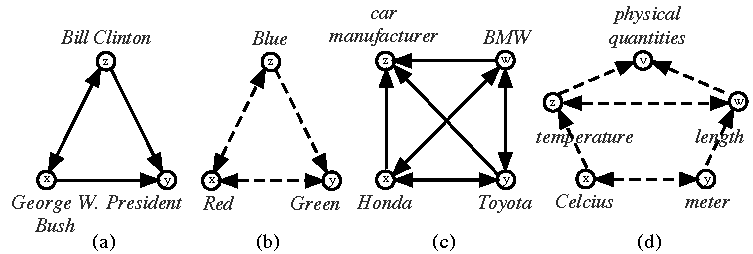
\includegraphics[totalheight=0.107\textheight]{networks}
  \caption{Examples of $n$-node concept networks with two
      input concept $x$ and $y$. Networks (a) and (c) show valid
      combinations of edges, whereas (b) and (d) are two relational
      constraints. For simplicity, we do not draw {\em no relation}
      edges in (d).}
  \label{fig:triangles}
\end{figure}

\subsection{Constraints as Prior Knowledge}
\label{sec:cons-prior-know}
Let $x, y$ be two input concepts, and $\mathcal{Z}=\{z_1, z_2, ...,
z_m\}$ be a set of additional concepts. For a subset $Z \in
\mathcal{Z}$, we construct a set of concept networks whose nodes are
$x$, $y$ and all elements in $Z$, and the edge, $e$, between every two
nodes is one of four taxonomic relations whose weight, $w(e)$, is
given by a local classifier (Sec. \ref{sec:learning}). If $l = |Z|$,
there are $n=2+l$ nodes in each network, and $4^{\left [ \frac{1}{2}
    n(n-1) \right ] }$ concept networks can be constructed. We only
focus on 3-node concept networks (i.e. $l = 1$). For example, for
input pair ({\em red}, {\em green}) and $\mathcal{Z} = \{ blue, yellow
\}$, we can construct 64 networks for triple $\left < red, green,
  Z=\{blue\} \right >$ and 64 networks for $\left < red, green,
  Z=\{yellow\} \right >$ by trying all possible relations between the
concepts.

\ignore{For a subset $Z \in \mathcal{Z}$, a set of concept networks is
  constructed. Each concept network contains two input concepts $x$,
  and $y$, and all additional concepts in $Z$. Every two concepts in a
  concept network are connected by their relations which are the four
  relations of interest in this paper. A local relation classifier is
  used to give weights for 4 relation classes of an edge in a concept
  network. We use $e$ and $w(e)$ to denote an edge in a concept
  network and its corresponding weight, respectively. If $n$ is the
  number of concepts in a network ($n > 2$), there will be $4^{\left [
      \frac{1}{2} n(n-1) \right ] }$ concept networks that can be
  constructed because there are $4$ relations for every $2$ concepts.
  With $m=1$, each network consists of 3 nodes, and there are $64$
  concept networks.}
%

A {\em relational constraint} is defined as a concept network, by
regarding only its edges' setting, that belongs to a pre-defined list
of invalid edges' combinations. For example, Figure
\ref{fig:triangles}b shows an invalid network where {\em red} is a
sibling of both {\em green} and {\em blue}, and {\em green} is an
ancestor of {\em blue}. In Figure \ref{fig:triangles}d, {\em Celcius}
and {\em meter} cannot be siblings because they are children of two
sibling concepts {\em temperature} and {\em length}. The relational
constraints used in our experiments are manually constructed.

\ignore{Figure \ref{fig:triangles}(b) demonstrates a relational
  constraint where the combination of edges is ({\em sibling}, {\em
    sibling}, {\em ancestor}) moving clockwise direction with respect
  to $x$ and $y$.}

Let $\mathcal{C}$ be a list of relational constraints. Equation (\ref{eqn:tscore}) defines the network scoring function,
which is a linear combination of the edge weights, $w(e)$, and the
penalties, $\rho_k$, of concept networks matching constraint $C_k \in
\mathcal{C}$.

\begin{equation}
  \label{eqn:tscore}
  score(t) = \sum_{e \in t} w(e) - \sum_{k=1}^{|\mathcal{C}|} \rho_{k} d_{C_k}(t)
\end{equation}

function $d_{C_k}(t)$ indicates if $t$ matches $C_k$. In our work, we
use relational constraints as hard constraints and set their penalty
$\rho_k$ to $\infty$. For a set of concept networks formed by $\left <
  x, y, Z \right >$ and all possible relations between the concepts,
we select the best network, $t^* = \text{argmax}_tscore(t)$.

\ignore{Eqn. \ref{eqn:tscore} allows us to pick the best
setting of all edges connecting concepts in the networks with respect
to $\mathcal{C}$.}

After picking the best concept network $t^*$ for every $Z \in
\mathcal{Z}$, we make the final decision on the taxonomic relation
between $x$ and $y$. Let $r$ denote the relation between $x$ and $y$
in a particular $t^*$ (e.g. $r = x \leftrightarrow y$.) The set of all
$t^*$ is divided into 4 groups with respect to $r$ (e.g. a group of
all $t^*$ having $r=x \leftrightarrow y$, a group of all $t^*$
having $r=x \leftarrow y$.) We denote a group with concept networks
holding $r$ as the relation between $x$ and $y$ by
$\mathcal{T}_{r}$. To choose the best taxonomic relation, $r^*$, of
$x$ and $y$, we solve the objective function defined in Equation
\ref{eqn:objectivefunction}.

\ignore{ After collecting all the topmost concept networks by going
  through all $Z \in \mathcal{Z}$, the topmost concept networks are
  divided into four groups with respect to the relation of $x$ and $y$
  in each network. Each group of the topmost concept networks is
  denoted by $\mathcal{T}_{r}$. To make the final decision
  concerning the relation of two input concepts $(x,y$), we solve the
  objective function defined in Eqn. \ref{eqn:objectivefunction}.}

\begin{equation}
  \label{eqn:objectivefunction}
  r^* = \text{argmax}_{r} \frac {1} {|\mathcal{T}_{r}|} \sum_{t^* \in \mathcal{T}_{r}} \lambda_{t^*} score(t^*)
\end{equation}

\ignore{
{\small
\begin{eqnarray}
\label{eqn:objectivefunction}
r^* & = & \text{argmax}_{r} \frac {1} {|\mathcal{T}_{r}|} \sum_{t \in \mathcal{T}_{r}} \lambda_{t} score(t) \\
& = & \text{argmax}_{r} \frac{1}{|\mathcal{T}_{r}|} \sum_{t \in \mathcal{T}_{r}} \lambda_{t} \left( \sum_{e \in t} w(e) - \sum_{k=1}^{|\mathcal{C}|} \rho_{k} d_{C_k}(t) \right) \notag
\end{eqnarray}
}
}

where $\lambda_t$ is the weight of concept network $t$, defined as the
occurrence probability of $t$ (regarding only its edges' setting) in
the training data, which is augmented with additional
concepts. Equation (\ref{eqn:objectivefunction}) finds the best
taxonomic relation of two input concepts by computing the average
score of every group of the best concept networks representing a
particular relation of two input concepts. \ignore{In general,
  $n$-node concept networks can be selected as relational constraints
  and used in our inference model. But one can always decompose
  $n$-node networks into $3$-node networks to allow greedy search in
  the concept network space.}

\ignore{

  To measure $\lambda_t$, a local relation classifier is used to
  predict the best relation between concepts in the concept networks
  in the training data.

  \begin{equation}
    \lambda_t = \frac{\# \text{ of occurrences of }t}{\# \text{ of
        predicted concept networks in training data}} \notag
  \end{equation}
}

\ignore{
\subsection{Constraint Selection}
\label{sec:constraintselection}

In Eqn. (\ref{eqn:objectivefunction}), a list of relational
constraints $\mathcal{C}$ is used. Recall that a relational constraint
is an invalid concept network that is not allowed to happen. In our
work, relational constraints are mined from the training data by
applying the {\em forward feature selection} technique discussed in
\cite{944968}. The algorithm starts with an empty set of constraints
$\mathcal{C}$, then grows the constraint set gradually by including in
the set the {\em best} concept network from each iteration. The {\em
  best} concept network is defined as the constraint used in
Eqn. (\ref{eqn:objectivefunction}) that improves the system's
performance most. Our {\em forward constraint selection} algorithm is
described in Figure \ref{alg:forwardselection}. Function
\texttt{evaluate}($\mathcal{D}$, $\mathcal{L}$, $\mathcal{C}$)
evaluates the system on all examples and their related concepts in
$\mathcal{D}$ using a trained local classifier $\mathcal{L}$ with
respect to a set of constraints $\mathcal{C}$ by solving the objective
function in Eqn. (\ref{eqn:objectivefunction})

\begin{figure}[!t]
  \begin{centering}
    {\scriptsize
      \fbox{
        \begin{minipage}{6in}
          \begin{tabbing}
            {Algorithm \textsc{Forward Constraint Selection}} \\
            \qquad {\textsc{Input}}: Data set with related concepts $\mathcal{D} = \left < (x, y, r, \mathcal{Z}) \right >$ ~~~~~\\
            \qquad \qquad A trained local relation classifier $\mathcal{L}$. \\
            \qquad \qquad A list of concept networks $\mathcal{T} = \{ t_1, t_2, \dots, t_{m} \}$; \\
            \qquad {\textsc{Output}}: Constraint set $\mathcal{C}$. \\
            \\
            \qquad $\mathcal{C} = \emptyset$; {\em isIncreasing} = true; \\
            \qquad {\em bestAcc} = \texttt{evaluate}($\mathcal{D}$, $\mathcal{L}$, $\mathcal{C}$); \\
            \qquad While ({\em isIncreasing}) do \\
            \qquad \qquad {\em isIncreasing} = false; \\
            \qquad \qquad For each $t \in \mathcal{T}$ do \\
            \qquad \qquad \qquad $\mathcal{C} = \mathcal{C} \cup \{ t \}$; \\
            \qquad \qquad \qquad {\em acc} = \texttt{evaluates}($\mathcal{D}$, $\mathcal{L}$, $\mathcal{C}$); \\
            \qquad \qquad \qquad If ({\em acc} $>$ {\em bestAcc}) then \\
            \qquad \qquad \qquad \qquad $t^* = t$; {\em isIncreasing} = true; \\
            \qquad \qquad \qquad \qquad {\em bestAcc} $=$ {\em acc}; \\
            \qquad \qquad \qquad End if \\
            \qquad \qquad \qquad $\mathcal{C} = \mathcal{C} \backslash \{ t \}$; \\
            \qquad \qquad End for \\
            \qquad \qquad If ({\em isIncreasing}) then \\
            \qquad \qquad \qquad $\mathcal{C} = \mathcal{C} \cup \{ t^* \}$; $\mathcal{T} = \mathcal{T} \backslash \{ t^* \}$; \\
            \qquad \qquad End if \\
            \qquad End while \\
            \\
            \qquad \textsc{Return}: $\mathcal{C}$; \\
          \end{tabbing}
        \end{minipage}
      }
    }
  \end{centering}
  \caption{
    \label{alg:forwardselection}
    Forward constraint selection algorithm. Function
    \texttt{evaluate}($\mathcal{D}$, $\mathcal{L}$, $\mathcal{C}$)
    evaluates the system on all examples and their related concepts in
    $\mathcal{D}$ using a trained local classifier $\mathcal{L}$ with
    respect to a set of constraints $\mathcal{C}$ by solving
    Eqn. (\ref{eqn:objectivefunction}).}
\end{figure}

One of the inputs of the algorithm, $\mathcal{T}$, is a set of $m$
concept networks. At each iteration, all concept networks $t \in
\mathcal{T}$ are tried; at the end of the iteration, the {\em
  best} network is added to $\mathcal{C}$ and removed from
$\mathcal{T}$. In this paper, for simplicity, we only use 3-node
concept networks, thus, $m = 64$. In general, $n$-node concept
networks can also be selected as relational constraints and used in
our model by decomposing $n$-node networks into $3$-node
networks to allow greedy search performed in the concept network
space.
}

\subsection{Extracting Related Concepts}
\label{sec:rel-con-ext}

To apply our constraint-based inference model, we need to acquire
concepts additional to the input pair. From now on, we refer to
additional concepts as {\em related concepts}. The related concept
space is defined as a space of direct ancestors, siblings and children
in a particular resource.

\ignore{In principle, with strong relational constraints and a
  reasonable local taxonomic relation classifier, one can use random
  concepts as additional concepts to do inference. However, there is a
  high chance that a random additional concepts will simply produce
  {\em no relation} with two input concepts, and eventually will not
  help the inference model.  \ignore{To address this issue, we
    investigate different approaches to obtain additional concepts
    which are related to input concepts.}  Our experiment (see
  Sec. \ref{sec:experiments} shows that the proposed inference model
  gets better results when doing inference with additional concepts
  that are more relevant to input concepts.}


\ignore{ In the first direction, as the first step to verifying the
  correctness of our proposed constraint-based inference model, we
  manually add {\em gold related concepts}, which are very related to
  input concepts. By using {\em gold related concepts}, a significant
  improvement in the system's performance is necessary to prove the
  correctness of the inference model. Our experiments (see
  Sec. \ref{sec:contr-relat-conc}) following this direction indeed
  prove that our proposed inference model is correct and accurate.  }

\begin{figure}[!t]
  \begin{centering}
    {\scriptsize
      \fbox{
        \begin{minipage}{6in}
          \begin{tabbing}
            \textsc{Yago} \textsc{Query Patterns} \\
            \qquad \textsc{Input:} concept ``$X$'' \\
            \qquad \textsc{Output:} lists of ancestors, siblings, and children of ``$X$'' ~~~~~~~~~~~~~~~~~~ \\
            \\
            \qquad \begin{tabular}{l|l|l}
              Pattern 1 & Pattern 2 & Pattern 3 \\
              \hline
              ``$X$'' \textsc{means} \texttt{?A} & ``$X$'' \textsc{means} \texttt{?A} & ``$X$'' \textsc{means} \texttt{?D} \\
              \texttt{?A} \textsc{subclassof} \texttt{?B} &  \texttt{?A} \textsc{type} \texttt{?B} & \texttt{?E} \textsc{type} \texttt{?D}  \\
              \texttt{?C} \textsc{subclassof} \texttt{?B} & \texttt{?C} \textsc{type} \texttt{?B} & \\
            \end{tabular}
            \\
            \\
            \qquad \textsc{Return:} \texttt{?B}, \texttt{?C}, \texttt{?E} as \\
            \qquad \qquad \qquad lists of ancestors, siblings, and children, respectively. \\
          \end{tabbing}
        \end{minipage}
      }
    }
  \end{centering}
  \caption{Our \textsc{Yago} query patterns used to obtain related concepts for ``$X$''.}
  \label{alg:yago-query}
\end{figure}

\ignore{However, in real world applications, {\em gold related
    concepts} are not available.}

We propose an approach that uses the \textsc{Yago} ontology
\cite{suchanek2007WWW} to provide related concepts. It is worth noting
that \textsc{Yago} is chosen over the Wikipedia category system used
in our work because \textsc{Yago} is a clean ontology built by
carefully combining Wikipedia and lexical database
WordNet.\footnote{However, \textsc{Yago} by itself is weaker than our
  approach in identifying taxonomic relations (see
  Sec. \ref{sec:experiments}.)}

In \textsc{Yago} model, all objects (e.g. {\em cities}, {\em people},
etc.)  are represented as {\em entities}. To map our input concepts to
entities in \textsc{Yago}, we use \textsc{means} relation defined in
\textsc{Yago} ontoloy. Furthermore, similar entities are grouped into
{\em classes}. This allows us to obtain direct ancestors of an entity
by using \textsc{type} relation which gives the entity's
classes. Furthermore, we can get ancestors of a class with
\textsc{subclassof} relation\footnote{These relations are defined in
  the \textsc{Yago} ontology.}. By using three relations
\textsc{means}, \textsc{type} and \textsc{subclassof} in \textsc{Yago}
model, we can obtain direct ancestors, siblings, and children, if any,
of an input concept. Figure \ref{alg:yago-query} presents three
patterns that we used to query related concepts from \textsc{Yago}
ontology. \ignore{For concepts having no children, such as {\em honda
    civic}, {\em bill clinton}, we simple ignore their children.}

% By default, we use this approach to provide related concepts for our
% constraint-based inference model.

\ignore{
\begin{figure}[!t]
  \begin{centering}
    {\scriptsize
      \fbox{
        \begin{minipage}{6in}
          \begin{tabbing}
            \textsc{Yago} \textsc{Query Patterns} \\
            \qquad \textsc{Input:} concept ``$X$'' \\
            \qquad \textsc{Output:} lists of ancestors, siblings, and children of ``$X$'' ~~~~~~~~~~~~~~~~~~ \\
            \\
            \qquad \textsc{Pattern 1:} \\
            \qquad \qquad ``$X$'' \textsc{means} \texttt{?A} \\
            \qquad \qquad \texttt{?A} \textsc{type} \texttt{?B} \\
            \qquad \qquad \texttt{?C} \textsc{type} \texttt{?B} \\
            \qquad \textsc{Pattern 2:} \\
            \qquad \qquad ``$X$'' \textsc{means} \texttt{?D} \\
            \qquad \qquad \texttt{?E} \textsc{type} \texttt{?D} \\
            \\
            \qquad \textsc{Return:} \texttt{?B}, \texttt{?C}, \texttt{?E} as \\
            \qquad \qquad \qquad lists of ancestors, siblings, and children, resp. \\
          \end{tabbing}
        \end{minipage}
      }
    }
  \end{centering}
  \caption{Our \textsc{Yago} query patterns used to obtain lists of direct ancestors,
    siblings, and children for concept $X$.}
  \label{alg:yago-query}
\end{figure}
}

\ignore{
In Figure \ref{alg:yago-query}, \textsc{Pattern 1} is used to get lists
of ancestors and siblings of a given concept.  For example, with
concept ``$X$''= ``{\em honda civic}'', \textsc{Pattern 1} returns
lists of ancestors \linebreak[4] \{{\em wikicat\_1970s\_automobiles,
  wn\_car\_102958343, \linebreak[4] wikicat\_Honda\_vehicles,
  $\dots$}\}, and siblings \linebreak[4] \{{\em Ford\_Capri,
  Mercury\_Comet, Honda\_Jazz, Honda\_Accord, $\dots$}\}. The prefix
and suffix annotation of the ancestors are dropped.  In the case that
ancestors are noun phrases, we only use the head of the phrase. We use
the Noun Group parser from \cite{suchanek2007WWW} to extract the {\em
  head} of a noun phrase. In the other hand, \textsc{Pattern 2}
returns an empty list of children of ``{\em honda civic}'', because
its corresponding entity \texttt{Honda\_Civic} is at the deepest level
in \textsc{Yago} ontology. The list of children will be non-empty if
``$X$'' is some generic concept such as ``{\em actor}'', ``{\em
  president}'', etc.
}

%%% Local Variables:
%%% mode: latex
%%% TeX-master: "jupiter"
%%% End:


\section{Experimental Study}
\label{sec:experiments}
In this section, we first describe the datasets. Follow that, we
present the experiments to evaluate our overall system and compare it
with other systems using existing large-scale resources. We also give
a deeper understanding about our system by performing several
experimental analyses.

\subsection{Datasets}
\label{sec:dataset}

In our experiments, two main datasets are used. The first dataset is
generated from 40 semantic classes of almost 11,000 instances. The
original semantic classes were manually constructed\footnote{Private
  communication.}  and was used to evaluate information extraction
tasks as in \cite{citeulike:1587018,pacsca-vandurme:2008:ACLMain}. The
second dataset is generated from 44 semantic classes of more than
10,000 instances used in
\cite{vyas-pantel:2009:NAACLHLT09}\footnote{There were 50 semantic
  classes in the original dataset. We grouped some semantically
  similar classes for the purpose of identifying taxonomic
  relations.}. The original classes of the second dataset were
extracted from Wikipedia lists. In both datasets, we have both types
of closed word semantic class (e.g. {\em chemical element}, {\em
  country}) and open word semantic class (e.g. {\em basic food}, {\em
  hurricane}). Moreover, there are classes with proper nouns
(e.g. {\em actor} with {\em Mel Gibson}) and classes with common nouns
(e.g. {\em basic food} with {\em rice}, {\em milk}).

Several semantic class names in the original data are written in a
short form (e.g. {\em chemicalelem}, {\em proglanguage}). We,
therefore, expand each semantic class name in the original dataset to
some meaningful names which are used by all systems in our
experiments. For example, {\em terroristgroup} is expanded to {{\em
    terrorist group}, {\em torrorism}}.

\begin{table}[!t]
  \small
  \centering
  \begin{tabular}{r|l|l}
    %\hline
    %\multicolumn{3}{|c|}{Concept pair examples} \\
    %\hline
    Relation          & Concept $X$ & Concept $Y$    \\
    \hline
    %\hline
    $X \leftarrow Y$        & actor             & Mel Gibson           \\
    & food              & rice                 \\
    % & wine              & Champagne            \\
    \hline                               
    $X \rightarrow Y$       & Makalu            & mountain             \\
    & Monopoly          & game                 \\
    % & krooni            & currency             \\
    \hline                               
    $X \leftrightarrow Y$   & Paris             & London               \\
    & copper            & oxygen                \\
    % & Nile              & Volga                 \\
    \hline                               
    $X \nleftrightarrow Y$ & Roja              & C++                  \\
    & egg               & Vega                  \\
    % & HotBot            & autism                \\
    %\hline
  \end{tabular}
  \caption{Some examples in our data set.}
  \label{table:examples}
\end{table}


We refer to both name of a semantic classes and its instances as
concepts. An example in the problem of taxonomic relation
identification is a pair of two concepts ($X$, $Y$) such as ({\em
  city}, {\em Dubai}), ({\em lead}, {\em aluminum}). We pair the
semantic classes and instances in the original data set to create
training and testing examples. For each original dataset, we randomly
generate disjoint training and test sets of $12,000$ and $8,000$
examples, respectively. We call the test set from the first and the
second datasets {\bf Test-I} and {\bf Test-II},
respecitively. \ignore{Because {\bf Test-II} contains only {\em
    Wikipedia concepts}, we do not evaluate it the experiments that
  find replacements for {\em non-Wikipedia concepts}.} Table
\ref{table:examples} shows some generated examples. All types of
taxonomic relations including $X \leftarrow Y$, $X \rightarrow Y$, $X
\leftrightarrow Y$, and $X \nleftrightarrow Y$ are covered with a
balanced number of examples.

To evaluate our system, we use a snapshot of Wikipedia from July,
2008. After cleaning up and removing articles without a category
(except redirect pages), and administrative articles such as {\em
  Template}, {\em Image} and {\em Portal} pages, there are 5,503,763
articles remained. We index these articles by using Lucene\footnote{http://lucene.apache.org, version
  2.3.2}.

\subsection{Overall Results and Comparison}
\label{sec:exp-results}

\ignore{
\begin{table*}[!t]
  \small
  \begin{center}
    \begin{tabular}{|l|c|c||c|c|}
      \hline
      \multirow{2}{*}{} & \multicolumn{2}{c}{{\bf Test-I}} & \multicolumn{2}{|c|}{{\bf Test-II}} \\
      \cline{2-5}
      &  Avg. Prec &  Avg. Rec &  Avg. Prec & Avg. Rec \\
      \hline
      Strube07  & 37.17 &  24.5 & 38.37 & 24.81 \\
      Snow06    & 50.12 & 40.19 & 41.27 & 32.19 \\
      Yago07    & 80.21 & 64.22 & 79.46 & 70.37 \\
      \hline
      {\bf Ours:}  & & & & \\
      ~~~RC        & 84.13 & 81.88 & 85.85 &  84.6 \\
      ~~~RC+BW     & 84.65 &  83.5 & 85.85 &  84.6 \\
      ~~~RC+Inf    & 85.36 & 83.33 & 87.82 & 86.87 \\
      ~~~RC+BW+Inf &  {\bf 85.9} &  {\bf 85.3} & {\bf 87.82} & {\bf 86.87} \\
      \hline
    \end{tabular}
    \caption{Evaluating and comparing performances, in average precision and recall, of the systems on {\bf
        Test-I} and {\bf Test-II}. There is no difference with {\bf BW} on {\bf Test-II} because {\bf Test-II} contains only {\em Wikipedia concepts}.}
    \label{table:compare-others}
  \end{center}
\end{table*}
}


To the best of our knowledge, no prior work directly targets the
problem of on-the-fly taxonomic relation identification. Most prior
work which relates to our problem focuses on building lexical taxonomy
or knowledge ontology \cite{Snow2006,wikitaxo07,suchanek2007WWW}. We
compare our system with three offline knowledge bases which are built
upon different existing resources.

{\bf Strube07} uses a large scale taxonomy which was derived from
Wikipedia \cite{wikitaxo07}, as the background knowledge. The taxonomy
was created by applying several lexical matching and methods based on
connectivity in the network to the category system in Wikipedia. The
taxonomy used in this system is in the latest version from March,
2008\footnote{Private communication.}. {\bf Snow06} uses the {\em
  augmented WordNet} \cite{ilprints665,Snow2006} as background
knowledge. To build the {\em augmented WordNet}, the authors first
identified lexico-syntactic patterns indicative of hypernymy from
corpora and use them to extract candidate noun pairs that may hold the
hypernym relation. Starting from WordNet-2.1 \cite{Fellbaum98}, the
latest version of the augmented WordNet has augmented 400,000
synsets. Words that are added into the augmented WordNet can be common
nouns or proper nouns. {\bf Yago07} uses \textsc{Yago} ontology
\cite{suchanek2007WWW} as the main source of background
knowledge. Because YAGO ontology is a combination of Wikipedia and
WordNet, this system is expected to be powerful in recognizing concept
relationships. To access a concept's ancestors and siblings, we use
patterns 1 and 2 in Fig. \ref{alg:yago-query} to move up on the
ontology from a concept. Our overall algorithm, {\bf TREI}, is
described in Fig. \ref{fig:rel-know-iden-alg}. We also evaluate our
local taxonomic relation classifier (Sec. \ref{sec:learning}),
which is referred as {\bf TREI (local)}. To make classification
decision with TREI (local), for a pair of concepts, we choose the
predicted relation with highest confidence returned by the classifier.

\begin{table}[!t]
  \begin{center}
    \begin{tabular}{l|c|c}
      &  {\bf Test-I}  &  {\bf Test-II}  \\
      \hline
      Strube07      &   24.32  &    25.63  \\
      Snow06        &   41.97  &    36.26  \\
      Yago07        &   65.93  &    70.63  \\
      \hline
      TREI (local)  &   81.89  &     84.7  \\
      TREI          &   {\bf 85.34}  &    {\bf 86.98}  \\
      %\hline
    \end{tabular}
    \caption{Evaluating and comparing performances, in accuracy, of
      the systems on {\bf Test-I} and {\bf Test-II}. \ignore{The best
        performance of each system, by varying the number of levels to
        go up on the taxonomy or category system, from $1$ to $4$, is
        reported.} TREI (local) uses only our local classifier to
      identify taxonomic relations by choosing the relation with
      highest confidence.}
    \label{table:compare-others}
  \end{center}
\end{table}

In all systems compared, we vary the value of $K$ from $1$ to $4$ as
the levels to go up to collect information in the taxonomy or category
tree. The best result of each system is reported. Table
\ref{table:compare-others} shows the comparison of all systems
evaluated on both {\bf Test-I} and {\bf Test-II}.  Our systems, as
shown, significantly outperform other systems implemented using
existing sophisticated resources.

\ignore{
Our overall system, which consists of
a taxonomic relation classifier ({\bf RC}), a component that finds
replacements ({\bf BW}) for {\em non-Wikipedia} concepts and an
inference component ({\bf Inf}), is referred as {\bf RC+BW+Inf} and
described in Fig. \ref{fig:rel-know-iden-alg}. We also evaluate our
system with only {\bf RC}, {\bf RC+Inf} and {\bf RC+BW}. In all
systems compared, we vary the value of $K$ from $1$ to $4$ as the
levels to go up to collect information in the taxonomy or category
tree. The best result of each system is reported. Table
\ref{table:compare-others} shows the comparison of all systems
evaluated on botah {\bf Test-I} and {\bf Test-II}. Note that we do not
find replacements for concepts in {\bf Test-II} as mentioned. Our
systems, as shown, significantly outperform other systems implemented
using existing sophisticated resources.
}

\subsection{Experimental Analysis}

In this section, we give some experimental analyses to understand
other aspects of our system.  \ignore{These analyses provide a deeper
  understanding of different aspects on our system.}

%\subsubsection{Performance on Individual Relation}

{\bf Performances on Individual Relation:} This experiment shows the
performance of our best system in Tab. \ref{table:compare-others} on
individual taxonomic relation.  Tab. \ref{tab:ind-rel} shows the
results in precision and recall.

\begin{table}[!t]
  \begin{center}
    \begin{tabular}{l|c|c||c|c}
      %\hline
      \multirow{2}{*}{TREI}  & \multicolumn{2}{c}{{\bf Test-I}} & \multicolumn{2}{|c}{{\bf Test-II}} \\
      \cline{2-5}
      &  Prec & Rec &  Prec &  Rec  \\
      \hline
      $X \leftarrow Y$       & 95.81 & 88.01 & 96.46 & 88.48 \\
      $X \rightarrow Y$      & 94.61 & 89.29 & 96.15 & 88.86 \\
      $X \leftrightarrow Y$  & 79.23 & 84.01 & 83.15 & 81.87 \\
      $X \nleftrightarrow Y$ & 73.94 &  79.9 & 75.54 & 88.27 \\
%      \hline
%      Average & & & & & & \\
      %\hline
    \end{tabular}
    \caption{Performance of our systems on individual taxonomic relation.}
    \label{tab:ind-rel}
  \end{center}
\end{table}

%\subsubsection{Evaluating on Special Datasets}

{\bf Evaluating on Special Datasets:} We evaluate the systems on
different dataset derived from {\bf Test-I}.  {\bf Test-I} consists of
$10,456$ concepts pairs with all concepts from Wikipedia and $1,544$
concept pairs with at least one {\em non-Wikipedia} concept.
Furthermore, if we only consider concepts pairs with all concepts from
WordNet and Wikipedia, there are $8,625$ pairs of interest.
Tab. \ref{table:special-data} shows the comparison of the systems on
these dataset which are denoted as {\bf Wikipedia}, {\bf
  non-Wikipedia} and {\bf WordNet}.  In this experiment, Yago07 gets
better results on {\bf Wikipedia} concept pairs than when evaluated
with {\bf Test-I}.  Snow06, as expected, gets better results on {\bf
  WordNet} concept pairs.  However, TREI still significantly
outperforms other systems. The improvement of TREI over TREI (local)
on the {\bf Wikipedia} and {\bf WordNet} datasets shows the
contribution of the constraint-based inference model. Whereas, the
improvement on {\bf non-Wikipedia} dataset shows the contribution of
function \texttt{findReplacement} (Sec. \ref{sec:overview-algorithm}).


\ignore{ By removing {\em non-Wikipedia concepts} from {\bf Test-I},
  we get $10,456$ concept pairs with concepts from {\bf
    Wikipedia}. From that, if we only consider concept pairs with
  concepts in WordNet, we have $8,625$ pairs. On the other hand, if we
  only consider {\em non-Wiki}. In {\bf Test-II}, we only have concepts
    in Wikipedia. By only consider pairs with concepts in WordNet, we
    have $7,830$ pairs, which makes {\bf Test-II-WN}.}

\ignore{
\begin{table}[!h]
  \small
  \begin{center}
    \begin{tabular}{|c||c|c|c|}
      %\hline
      %\multicolumn{5}{|c|}{Comparison on special data sets} \\
      \hline
      & {\bf Test-I-WK} & {\bf Test-I-WN} &  {\bf Test-II-WN}  \\
      \hline
      Strube07   & 24.59 & 24.13 & 26.49 \\
      Snow06     & 41.23 & 46.91 & 43.07 \\
      Yago07     & 69.95 & 70.42 & 70.37 \\
      {\bf Ours} & {\bf 91.03} &  {\bf 91.2} & {\bf 86.29} \\
      \hline
    \end{tabular}
    \caption{Performance, in accuracy, of the systems.}
    \label{table:special-data}
  \end{center}
\end{table}
}

\begin{table}[!t]
  \small
  \begin{center}
    \begin{tabular}{l|c|c|c}
      &  {\bf Wikipedia}  & {\bf WordNet}  &  {\bf non-Wikipedia}  \\
      \hline
      Strube07  &      24.59         &     24.13      & 21.18                 \\
      Snow06    &      41.23         &     46.91      & 34.46                 \\
      Yago07    &      69.95         &     70.42      & 34.26                 \\
      \hline
      TREI (local) &   89.37         &     89.72      & 31.22                 \\
      TREI      &      {\bf 91.03}   &     {\bf 91.2} & {\bf 45.21}           \\
      %\hline
    \end{tabular}
    \caption{Performance of the systems on special datasets, in
      accuracy. For all concept pairs from {\bf non-Wikipedi}, TREI
      (local) simply returns sibling relation.}
    \label{table:special-data}
  \end{center}
\end{table}


%\subsubsection{Contribution of Related Concepts in Inference}
%\label{sec:contr-relat-conc}
{\bf Contribution of Related Concepts in Inference:} In this
experiment, we show the results of TREI when using another source than
\textsc{Yago} to provide related concepts to the constraint-based
inference model.  We use the original data from
\cite{pacsca-vandurme:2008:ACLMain}, which was used to generate {\bf
  Test-I}. For each concept in an input pair from {\bf Test-I}, we get
its ancestors, siblings, children, if any, from the original data and
use them in the inference process. This system is referred as TREI
(Gold Inf.). Tab. \ref{table:related-concepts} present the results of
TREI and TREI (Gold Inf.) on different $K$ as the number of levels to
go up on the Wikipedia category.
We see that {\bf TREI} gets better results when doing inference with
better related concepts. In this experiment, two systems use the same
number of related concepts.

\begin{table}[!t]
  \small
  \begin{center}
    \begin{tabular}{l|c|c|c|c}
      &    $K$=1  &    $K$=2  &    $K$=3  &    $K$=4  \\
      \hline
      TREI             &  82.93  &  85.34  &  85.23  &  83.95  \\
      TREI (Gold Inf.)  &  83.46  &  86.18  &   85.9  &  84.93  \\
    \end{tabular}
    \caption{Evaluating TREI with different sources providing related
      concepts to do inference. $K$ is the number of levels to go up
      on the Wikipedia category.}
    \label{table:related-concepts}
  \end{center}
\end{table}

\ignore{
\begin{figure}[t]
  \centering
  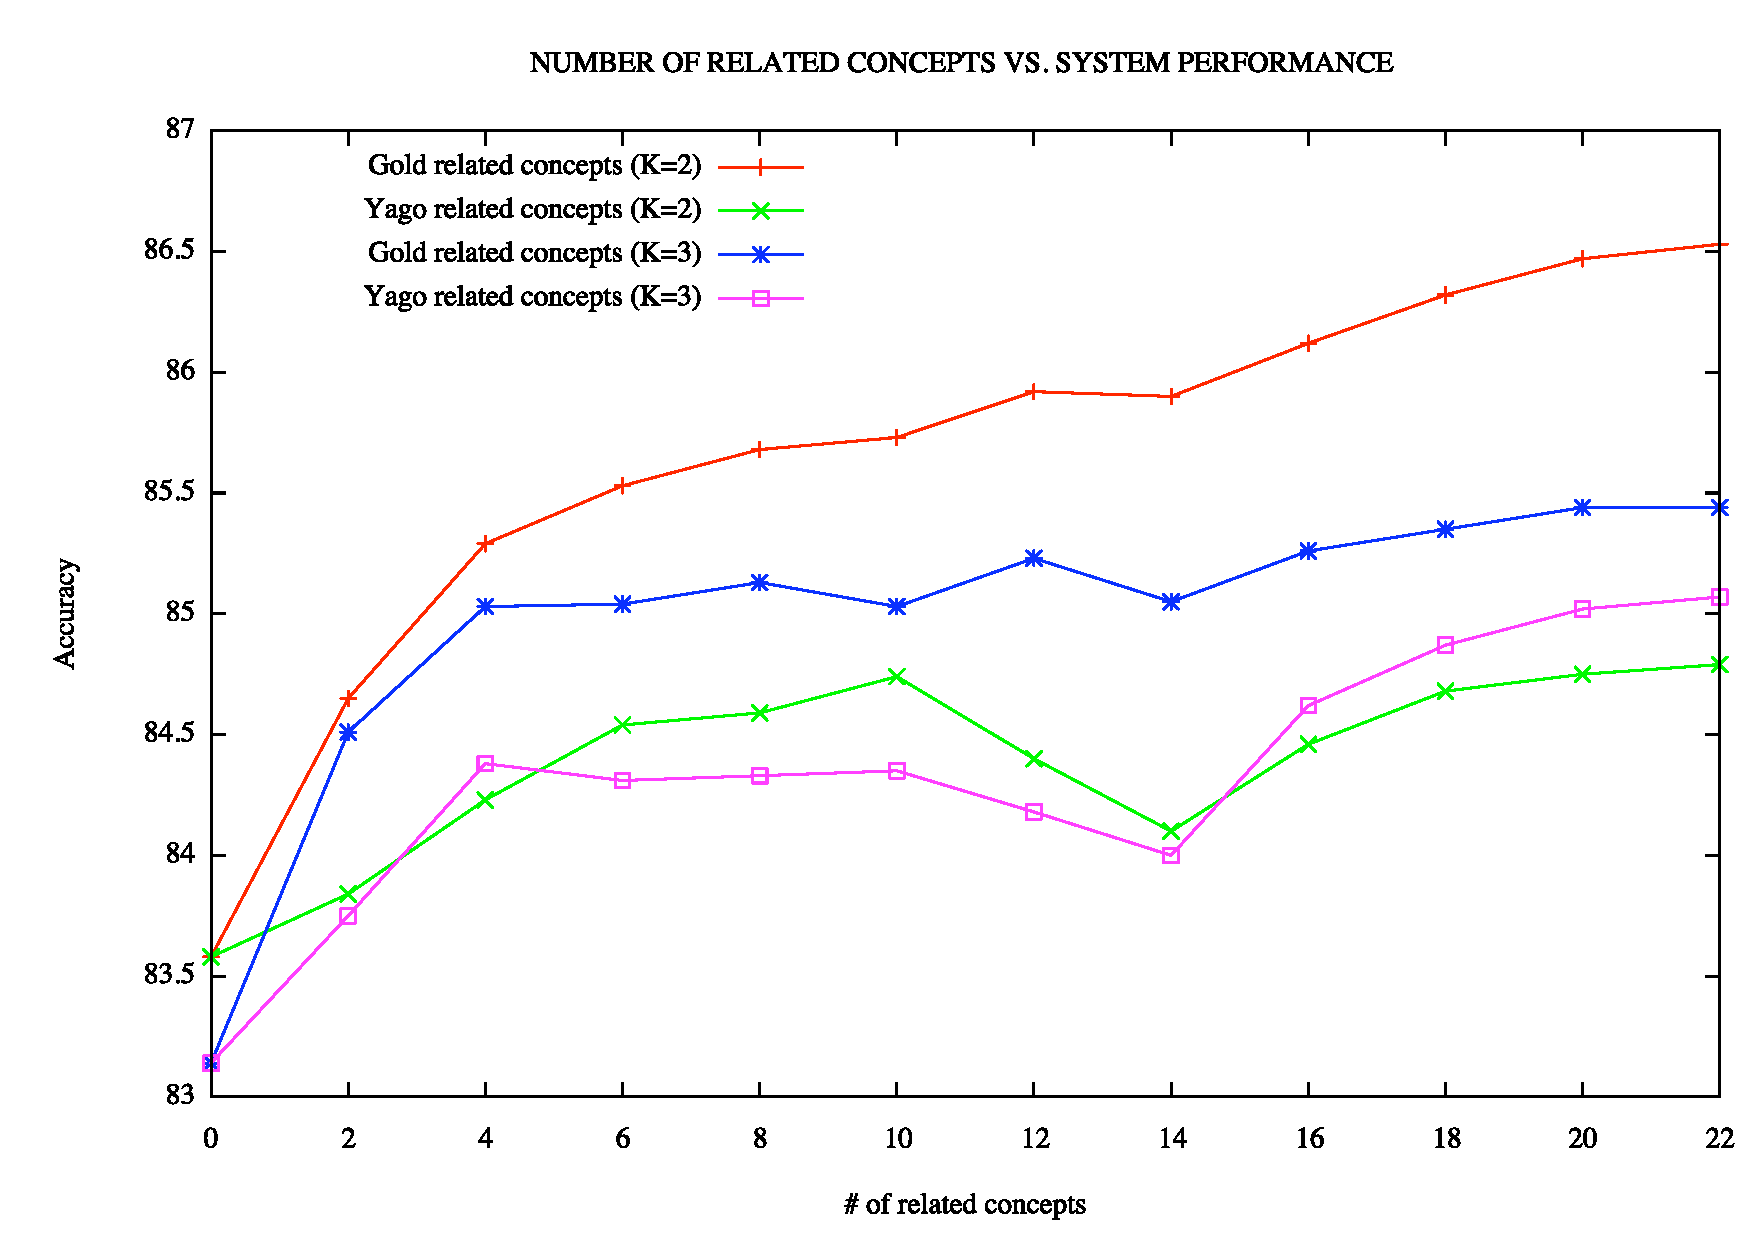
\includegraphics[totalheight=0.21\textheight]{relatedconcepts4}
  \caption{Relation between our system performance and the number of
    related concepts used in the constraint-based inference model.}
  \label{fig:related-concepts}
\end{figure}
}

\ignore{ In Sec. \ref{sec:rel-con-ext},  we propose the intuition that
  the more  relevant to the  input concepts the related  concepts are,
  the  better performance  the  system gets.  In  this experiment,  we
  empirically show the correctness  of the intuition by evaluating our
  best    system    with    inference    model   on    {\bf    Test-I}
  dataset.  Fig. \ref{fig:related-concepts} shows  the results  of the
  systems using  the inference  model with related  concepts extracted
  from the original dataset and from \textsc{Yago}.  }

%%%%%%%%%%%%%%%
% Old writing %
%%%%%%%%%%%%%%%

\ignore{Specifically, examples are created with the following
  guidelines.

  \begin{itemize}
  \item $X \leftarrow Y$ examples: For each semantic class, we pair
    the name of the class with its instances. These examples have the
    general form ({\em semantic class X}, {\em child of X}).
  \item $X \rightarrow Y$ examples: These examples have the general
    form ({\em concept X}, {\em semantic class of X}).
  \item $X \leftrightarrow Y$ examples: The general form of these
    examples is ({\em concept X}, {\em concept Y}), where $X$ and $Y$
    are two instances of a semantic class, and $X \ne Y$.
  \item $X \nleftrightarrow Y$ examples: To make examples with two
    concepts having no relation, we pair either a semantic class name
    and an instance of another semantic class (and vice versa), or an
    instance in a semantic class and another instance in other
    classes.
  \end{itemize}
}

\ignore{We refer to the 12,000-example test set as the {\em TestAll}
  test set. From the training set, we discard examples with one or
  both concepts not in Wikipedia ({\em non-Wikipedia examples}). This
  results in a training set of $6,959$ examples.  It is important to
  note that, we do not discard {\em non-Wikipedia} examples in the
  {\em TestAll} test set. Table \ref{tab:detail-dataset} shows the
  statistics of the training and test data.

  \begin{table}[!t]
    \small
    \begin{center}
      \begin{tabular}{|l||c|c|c|c|c|}
        \hline
        Data & $X \leftarrow Y$ & $X \rightarrow Y$  & $X \leftrightarrow Y$  & $X \nleftrightarrow Y$ & Total \\
        \hline
        \hline
        {\em Training}  & 1,739 & 1,754 & 1,664 & 1,802 & 6,959\\
        % {\em TestWiki} & 2,684 & 2,654 & 2,483 & 2,635 & 10,456 \\
        {\em TestAll} & 3,045 & 3,025 & 2,965 & 2,965 & 12,000 \\
        \hline
      \end{tabular}
      \caption{Details of the training and test sets with the number
        of examples in each relation class. The {\em Training} set
        contains only examples in Wikipedia. {\em TestAll} includes
        {\em non-Wikipedia} examples.}
      \label{tab:detail-dataset}
    \end{center}
  \end{table}
}

\ignore{Each semantic class is an incomplete set of representative
  instances and has about 272 instances in average. The smallest class
  is {\em search engine} with 25 instances, and the largest class is
  {\em actor} with 1500 instances. Table \ref{table:class-instance}
  shows a snippet of the dataset. We have both types of closed word
  semantic class (e.g. {\em chemical element}, {\em country}) and open
  word semantic class (e.g. {\em basic food}, {\em
    hurricane}). Moreover, there are classes with proper nouns
  (e.g. {\em actor} with {\em Mel Gibson}) and classes with common
  nouns (e.g. {\em basic food} with {\em rice}, {\em milk}).

  \begin{table}[!t]
    \small
    \centering
    \begin{tabular}{|r|l|}
      \hline
      \multicolumn{2}{|c|}{A snapshot of the original dataset} \\
      \hline
      \textbf{Semantic class (Size)} & \textbf{Examples of Instances} \\
      \hline
      \hline
      basic food (155) & rice, milk, eggs, beans, fish \\
      \hline
      chemical element (118) & lead, copper, aluminum, calcium \\
      \hline
      city (589) & San Francisco, Dubai, Chicago \\
      \hline
      disease (209) & arthritis, hypertension, influenza \\
      \hline
      actor (1500) & Kate Hudson, Mel Gibson \\
      \hline
    \end{tabular}
    \caption{A snippet of 40 semantic classes with instances. 
      The class names in the original dataset ({\em basicfood}, 
      {\em chemicalelem}) were presented in a meaningful form
      as shown in the left column.}
    \label{table:class-instance}
  \end{table}
}

\ignore{ Lucene is a high-performance text search library written in
  Java and widely used as an off-the-shelf IR system.}

\ignore{
  \begin{table}[!t]
    \small
    \begin{center}
      \begin{tabular}{|c||c|c|c|c|}
        \hline
        \multicolumn{5}{|c|}{Overall results and comparison} \\
        \hline
        $K$  &  \textsc{Strube 07}  &  \textsc{Snow 06}  &  \textsc{Yago 07}  &  \textsc{Ours}            \\
        \hline
        1  &      23.83  &    40.24  &           64.43  &  \textbf{82.13}  \\
        2  &      23.84  &    42.63  &           63.94  &  \textbf{84.79}  \\
        3  &      23.88  &    40.96  &           62.02  &  \textbf{85.07}  \\
        4  &      24.32  &    40.65  &           60.57  &  \textbf{84.08}  \\
        \hline
      \end{tabular}
      \caption{Performance of our overall system compared to other
        systems. Performances are measured by accuracy. The {\em
          TestAll} test set with $12,000$ examples is used in this
        experiment. $K$ is the number of levels to climb up in the
        hierarchical structure of knowledge sources as described in the
        text.}
      \label{table:compare-others}
    \end{center}
  \end{table}
}

\ignore{Our system also uses Wikipedia as its main background
  knowledge. However, ours is superior to other systems because it
  employs advance machine learning techniques along with a powerful
  and effective constraint-based inference model.}

\ignore{
  \begin{enumerate}

  \item \textsc{Strube 07} uses a large scale taxonomy which was
    derived from Wikipedia \cite{wikitaxo07}, as the background
    knowledge. The taxonomy was created by applying several lexical
    matching and methods based on connectivity in the network to the
    category system in Wikipedia. As a result, the taxonomy contains a
    large amount of subsumption, i.e. {\em isa}, relations
    \cite{wikitaxo07}. Given an input with two concepts $X$ and $Y$,
    using the taxonomy, $X$ is an ancestor of $Y$ if one of the
    articles about $Y$ is subsumed by an article about $Y$, using {\em
      isa} links of articles, up to $K$ levels in the taxonomy.
    Similarly, for the case that $Y$ is an ancestor of $X$. If $X$ and
    $Y$ share a common ancestor within $K$ levels in the taxonomy,
    they are considered siblings. We first apply our concept
    disambiguation algorithm on given concepts and then mount them
    onto the taxonomy to infer the relations. The taxonomy used in
    this experiment is in the latest version from March,
    2008\footnote{Private communication with Michael Strube and Simone
      Paolo Ponzetto, 2009.}.

  \item \textsc{Snow 06} uses the {\em augmented WordNet}
    \cite{ilprints665,Snow2006} as background knowledge. To build the
    {\em augmented WordNet}, the authors first identified
    lexico-syntactic patterns indicative of hypernymy from corpora and
    use them to extract candidate noun pairs that may hold the
    hypernym relation. A trained classifier is applied on these noun
    pairs to recognize the pairs holding hypernym relation. Starting
    from WordNet-2.1 \cite{Fellbaum98}, the latest version of the
    augmented WordNet has augmented 400,000 synsets. Words that are
    added into the augmented WordNet can be common nouns or proper
    nouns. The augmented WordNet can serve as effective background
    knowledge for identifying the relational knowledge of interest by
    looking for the input concepts in the augmented WordNet tree in all
    possible senses of the concepts and then inferring their
    relationship. We also vary the value of $K$ as the number of
    levels to go up on the WordNet tree from input concepts to find
    their common subsumptions.

  \item \textsc{Yago 07} uses YAGO ontology \cite{suchanek2007WWW} as
    the main source of background knowledge. Because YAGO ontology is
    a combination of Wikipedia and WordNet (see our brief description
    in Sec. \ref{sec:rel-con-ext}), this system is expected to be
    powerful in recognizing concept relationships. To access a
    concept's ancestors and siblings, we combine \textsc{Pattern 1} in
    Fig. \ref{alg:yago-query} and the \textsc{subClassOf} relation in
    YAGO model to go up on the ontology. The \textsc{subClassOf}
    relation can be cascaded $K$ times to climb up in the ontology.

  \end{enumerate}
}

\ignore{
Because the systems in the previous experiments do not use the same
source of background knowledge, we, furthermore, perform experiments
in which these systems are compared with different data sets covered
in different knowledge sources. This experiment provides a fair
comparison for systems that use different resources as their
background knowledge. New data sets are derived from the {\em TestAll}
test set. The first derived data set is {\em TestWiki} which contains
only {\em Wikipedia concepts}. By removing all examples with {\em
  non-Wikipedia concept}, there are $10,456$ examples remained in {\em
  TestWiki}. The second derived data set is {\em TestWn}, which
contains only concepts in the {\em augmented WordNet}
\cite{ilprints665,Snow2006}.  {\em TestWn} has $8,625$ examples after
dropping $3,375$ examples with concepts not in the {\em augmented
  WordNet} from {\em TestAll}.  The results of this experiment are
shown in Tab. \ref{table:exp-diff-test}.  We only report the best
results achieved by the systems on different test sets. Our system
still significantly outperforms other systems when compared on
specific data sets.

\begin{table}[!t]
  \small
  \begin{center}
    \begin{tabular}{|c||c|c|c|c|}
      \hline
      \multicolumn{5}{|c|}{Comparison on special data sets} \\
      \hline
      Data set &  \textsc{Strube 07}  &  \textsc{Snow 06}  &  \textsc{Yago 07}  &  \textsc{Ours}   \\
      \hline
      {\em TestWiki}  &               24.59  &             44.34  &             70.29  &  \textbf{90.92}  \\
      {\em TestWn}    &               24.13  &             47.79  &             70.81  &  \textbf{90.76}  \\
      \hline
    \end{tabular}
    \caption{Comparison of systems' performance with different test
      sets derived from the {\em TestAll} test set. {\em TestWiki}
      contains $10,456$ examples in Wikipedia, and {\em TestWn}
      contains $8,625$ examples in the {\em augmented WordNet}. The
      best performance of each system (by varying $K$) is reported.}
    \label{table:exp-diff-test}
  \end{center}
\end{table}
}

\ignore{
\begin{table*}[!t]
  \begin{center}
    \begin{tabular}{|l||c|c|c|}
      \hline
      \multicolumn{4}{|c|}{Constribution of the components in our system} \\
      \hline
      &         Results on $10,456$  &  Results on $1,544$              &         Overall results  \\
      System &  {\em Wikipedia examples}  &  {\em non-Wikipedia examples}  &  on $12,000$ examples  \\
      \hline
      \hline
      Baseline        &                       88.79  &                      31.22       &                   81.38  \\
      \hline
      w/o Inference   &                       88.79  &                      44.88       &                   83.14  \\
      \hline
      with Inference  &                       \textbf{90.92}  &                      \textbf{45.40}       &                   \textbf{85.07}  \\
      \hline
    \end{tabular}
    \caption{\small Contributions of the components in our system evaluated
      on three types of data. The first column shows results only on
      examples with concepts that appear in Wikipedia. The second
      column shows results on examples having concepts that do not
      appear in Wikipedia, and thus exhibits the power of our method
      to extend outside Wikipedia. The third column shows results on
      the overall data set, that consists of around 13\% of the
      concepts pairs that are outside Wikipedia. The {\em Baseline}
      system is our local relation classifier that uses neither the
      approach of finding replacements for {\em non-Wikipedia
        concepts} nor the inference model. The baseline on {\em
        non-Wikipedia examples} is computed by assuming sibling
      relation all the time. By adding the component of finding
      replacements for {\em non-Wikipedia concepts}, we have the {\em
        w/o Inference} system.}
    \label{tab:w-wo-infer}
  \end{center}
\end{table*}
}


\ignore{
  \subsubsection{Contributions of the Components in our System}

  In this experiment, we show the contribution of the components in
  our overall algorithm (see Fig. \ref{fig:rel-know-iden-alg}). We use
  different data sets in this experiments to study the variation in
  behavior of our system. The first data set is the {\em TestWiki} in
  the previous experiment. This test set contains $10,456$ examples
  with {\em Wikipedia concepts}. These are the remained examples after
  dropping {\em non-Wikipedia concepts} from $12,000$ examples in the
  {\em TestAll} test set. The second test set contain only $1,544$
  concept pairs with at least one {\em non-Wikipedia} concept in
  each. In other words, the second test set is the complement of the
  {\em TestWiki} test set with respect to the {\em TestAll} test
  set. The third test set is the {\em TestAll} test set. The results
  are shown in Tab. \ref{tab:w-wo-infer}.

  In Tab. \ref{tab:w-wo-infer}, the {\em Baseline} system is our local
  relation classifier that uses neither the component finding
  replacements for {\em non-Wikipedia concept} nor the
  constraint-based inference model. The baseline on {\em non-Wikipedia
    examples} is computed by assuming sibling relation all the
  time. In the {\em w/o Inference} row, we evaluate our system with
  the contribution of the component finding replacements for {\em
    non-Wikipedia concepts}, but inference model. The result on
  $10,456$ {\em Wikipedia examples} remains the same because, all of
  concepts in these examples are in Wikipedia, the system does not
  need to find replacement concepts. The significant improvement in
  the results on $1,544$ {\em non-Wikipedia examples} shows the
  effectiveness of our approach in finding replacements for {\em
    non-Wikipedia concepts}. Overall, we obtain almost $2\%$ of
  improvement in accuracy after adding the finding replacement
  component. The third experiment is carried out by evaluating our
  overall algorithm in Fig. \ref{fig:rel-know-iden-alg} on all test
  sets. The inference process significantly improve the results of our
  system on $10,456$ {\em Wikipedia examples}. It also gains
  improvements on the {\em non-Wikipedia examples} so that in overall,
  by adding the constraint-based inference component, the system
  improves $\sim 2\%$ in accuracy. Overall, our system achieves
  significant improvement reaching to $85.07\%$ accuracy in overall by
  adding in all components, compared to $81.38\%$ accuracy gained by
  the {\em Baseline} system.

  \begin{table*}[!t]
    \small
    \begin{center}
      \begin{tabular}{|c|c|c|c|c|c|c|c|}
        \hline
        No.  &  $X$             &  $Y$          &  True    &  LocalClassifier       &  \multicolumn{2}{|c|}{Replacement Needed?}  &  withInference \\ \cline{6-7}
        &                  &               &  Label   &  Prediction                   &  $X$                  &  $Y$                     &  Prediction           \\
        \hline
        \hline
        1&city                    &lisbon                   &$X \leftarrow Y$      &$X \leftarrow Y$      &(no)        &(no)         &$X \leftarrow Y$  \\
        2&{\em bartlomiej strobel}&painter                  &$X \rightarrow Y$     &$X \rightarrow Y$     &drew struzan&(no)         &$X \rightarrow Y$ \\
        3&taiwan                  &singapore                &$X \leftrightarrow Y$ &$X \leftarrow Y$               &(no)        &(no)         &$X \leftrightarrow Y$ \\
        4&jean ingres             &{\em harald slott-moller}&$X \leftrightarrow Y$ &$X \nleftrightarrow Y$         &(no)        &george inness&$X \leftrightarrow Y$ \\
        5&{\em southern herald}   &newspaper                &$X \rightarrow Y$     &$X \leftrightarrow Y$          &liberty     &(no)         &$X \rightarrow Y$  \\
        6&somalia                 &hurricane                &$X \nleftrightarrow Y$&$X \nleftrightarrow Y$&(no)        &(no)         &$X \leftrightarrow Y$  \\
        \hline
      \end{tabular}
      \caption{Relationship prediction examples from {\em TestAll}
        test set. Concepts in {\em italic font} are not in Wikipedia,
        and they are replaced by other {\em Wikipedia concepts} as
        shown.}
      \label{table:pre-examples}
    \end{center}
  \end{table*}
}

\ignore{
In our inference process, we used related concepts added to form
relational constraints in concept networks. The relational constraints
will then enforce concept networks to eliminate violated ones and pick
the best concept network available. From our inference model, we make
two following claims: (1) The more relevant to the input concepts the
related concepts are, the better performance the system gets, and (2)
the more related concepts added to the inference process, the better
performance the system gets.

To prove the first claim, we use the original data of forty semantic
classes (see Sec. \ref{sec:dataset}) to provide {\em gold related
  concepts} to the inference process as discussed in
Sec. \ref{sec:rel-con-ext}. Our experiment shows that by using this
approach, the performance of our best system reaches to $86.52\%$ in
accuracy on the {\em TestAll} test set, compared to $85.07\%$ accuracy
obtained when using another knowledge source to provide related
concepts. For the second claim, we evaluate our system with several
numbers of related concepts added to the inference process. In this
experiment, we use both the {\em gold related concepts} provided by
the original dataset and the {\em YAGO related concepts} extracted
from YAGO ontology (see Sec. \ref{sec:rel-con-ext}) for the inference
process.

Fig. \ref{fig:related-concepts} shows the improvement in the
performance of our system with respect to the quality of the related
concepts used and also the number of related concepts. This experiment
is done on the {\em TestAll} test set. It is shown clearly that the
related concepts from gold data outperform the related concepts
extract from the other source. Due to the quality of the related
concepts extracted from YAGO ontology, sometimes, adding more concepts
hurts the performance. We use $K=2$ and $K=3$ in this
experiment\footnote{$K$ is the number of levels to go up in the
  Wikipedia category system to extract features for input concept
  pairs.}. The related concepts include the ancestors, siblings, and
children of an input concept. For simplicity, in this experiment we
only report the total number of related concepts extracted for two
input concepts of an example.
}

\ignore{
  \subsubsection{System's Output Examples}

  Table \ref{table:pre-examples} shows some output examples of our
  overall system in Fig. \ref{fig:rel-know-iden-alg} (see column {\em
    withInference}). We also present the predictions made by the
  system without inference component ({\em LocalClassifier}). Concepts
  which are not in Wikipedia will be replaced by {\em Wikipedia
    concepts} ({\em Replacement Needed?}). Example \#1 and \#2 show
  two concept pairs correctly classified by both {\em LocalClassifier}
  and {\em with Inference}. Especially, in \#2, that concept {\em
    bartlomiej strobel} is replaced with {\em drew struzan} helps the
  systems make correct predictions. In examples \#3, {\em
    LocalClassifier} make incorrect predictions, but {\em
    withInference} remedies this. Example \#4 and \#5 show two cases
  where two {\em non-Wikipedia concepts} are correctly replaces with
  two corresponding {\em Wikipedia concepts}, but {\em
    LocalClassifier} still makes incorrect prediction. However, {\em
    withInference}, with its power of internal reasoning using
  relational constraints, proves to be successful. Example \#6 is an
  example where {\em LocalClassifier} makes correct prediction, but
  {\em withInference} does not. This is probably because of bad
  related concepts extracted for the two input concepts.  }


%%% Local Variables: 
%%% mode: latex
%%% TeX-master: "jupiter"
%%% End: 


\section{Related Work}
\label{sec:related-work}
To the best of our knowledge, no previous study has directly addressed
the problem of identifying taxonomic relation between two given
concepts. However, there are several work which acquires structured
taxonomies and ontologies.

\ignore{Several lines of work share similarities to the work presented
  here. One line of work makes use of the web and exploits the fact
  that many relations are expressed explicitly and locally, typically
  within a single sentence. It uses this to discover terms which have
  hypernyms or coordinate relations \cite{citeulike:282193,Snow2006}
  or to expand or refine members in a semantic class (given seeds or
  the semantic class itself)
  \cite{WangCohen09,VyasPantel09,kozareva-riloff-hovy:2008:ACLMain,4470258,banko-etzioni:2008:ACLMain}.
  A second line of work attempts to classify pre-specified relations
  \cite{citeulike:454000,Sekine06,RothYi04} and typically makes use of
  supervised or semi-supervised learning techniques.

  The later line of work is different from ours in terms of goals and
  techniques. It considers relations such as ``SpouseOf" of ``BornIn"
  and relies on the relation being expressed in close proximity,
  typically within a sentence, and on training supervised classifiers.
  The line of work which makes use of the web is similar to ours in
  terms of the final task, but is different in its assumptions and
  techniques---it mostly relies on the fact that due to redundancy of
  information in the web, and presumes that many related terms will appear often
  enough in some simple explicit form in close proximity.}

In \cite{ilprints665} and \cite{Snow2006}, the authors constructed
classifiers to identify hypernym relationship between concepts. The
classifiers is then used to augment WordNet \cite{Fellbaum98} with
over $400,000$ synsets. 

\ignore{ They combine their hypernym-only classifier and the
  ($m$,$n$)-cousin classifier with the evidence features to recognize
  the hypernym and cousin relationships among nouns.  Their inferred
  taxonomy achieves the best performance after adding 30,000 novel
  hyponyms compared to those in WordNet-2.1.  They show that their
  system relatively improves F-score by 23\% over the WordNet-2.1
  hypernym classifier.}

\ignore{ Using similar techniques to the aforementioned line of work,
  there has been a large body of work on automatically expanding a set
  of entities given some seeds that belong to a semantic class or the
  class itself. A typical application of this research is that of
  expanding, correcting or refining Google
  Sets\footnote{http://labs.google.com/sets}.

%
  % The common input of systems in this direction is a set of seeds in
  % a particular semantic class that one wishes to get other members
  % of that class.
%
  Typically, these methods search the web for patterns around the
  seeds and bootstrap to other semantically similar members of the
  class~\cite{kozareva-riloff-hovy:2008:ACLMain,talukdar-EtAl:2006:CoNLL-X}.
  Alternatively, \cite{4781230,4470258} use the surrounding contexts
  of the seeds in semi-structured text to extract other members of the
  set. Similarly,
  \cite{citeulike:1587018,pacsca-vandurme:2008:ACLMain} automatically
  acquire open-domain classes of entities and attributes by using
  very little supervised seed information.
  % Web documents and query logs are used in the acquisition process.
}

\ignore{The key difference between this line of work and the approach
  we develop here is that we are given two concepts and must determine
  the relation between them. The coverage of the aforementioned
  methods is lacking since they rely on concepts appearing in close
  proximity with specific patterns that reveal their relation. It is
  likely, however, that our input concepts never occur together in a
  given sentence even though they are clearly related. As we
  show, we can robustly and accurately determine these relations,
  significantly outperforming state of the art acquisition methods
  such as \cite{Snow2006}.}

\cite{wikitaxo07} generated a taxonomy using Wikipedia as the
knowledge source. They used the Wikipedia category system as a
conceptual network consisting of subsumption ({\em isa})
relations. \cite{suchanek2007WWW} presented the the \textsc{Yago}
ontology, which was automatically constructed using both Wikipedia and
WordNet. The \textsc{Yago} approach built on the {\em infoboxes} and
{\em category pages} in Wikipedia and linked to a clean taxonomy of
concepts in WordNet. \textsc{Yago} provides many useful relations such
as {\em subClassOf}, {\em bornOnDate}, and {\em type}.  Our work
differs from this line of work because we do not build a knowledge
base, but rather directly identify taxonomic relations between two
given concepts.

% % Story of previous work

% % 1. Summarize the work on discovering terms which have hypernym or
% % coordinate relation. E.g. the work of Marti Hearst 1992, Rion Snow
% % 2006, Hovy 2005.

% % 2. Summarize the work about expanding sets and refining set
% % expansion. E.g. the work of Cohen 2007, 2008, 2009, Hovy 2007, Pasca
% % 2007, 2008, Sarmento 2007, Pantel 2009

% % 3. Perhaps also summarize the work of relation classifiercaiton. E.g. Zhu Zhang 2004, 

% % 4. Claim that other work using supervised learning with pre-defined
% % list of relation and domain dependency, we do different things: (a)
% % supervised learning with arbitrary types of ancestor and cousin
% % relations, (b) we are domain-independent: train on some domains and
% % work well in other domains. This is also the contributions of this
% % paper.

% The task of relational knowledge identification can be seen as related
% to the work on discovering terms which have hypernym or coordinate
% relation \cite{citeulike:282193,Snow2006}, expanding or refining sets
% of a semantic class from a list of given seeds or the semantic class
% itself
% \cite{WangCohen09,VyasPantel09,kozareva-riloff-hovy:2008:ACLMain,4470258},
% or classifying pre-specified relations \cite{citeulike:454000}.

% In \cite{ilprints665}, the authors construct a hypernym-only
% classifier using the dependency path patterns discovered in the
% sentences that contain noun pairs in hypernym and hyponym
% relations. Furthermore, they show that using coordinate terms can help
% improve the recall of the hypernym classifier. The best system in
% their work is a hypernym-only classifier additionally trained with
% hundred thousands of dependency paths extracted from the Wikipedia corpus.
% The system outperforms the best WordNet classifier in identifying
% coordinated terms by relatively improving F-score by over
% 54\%. Recently, \cite{Snow2006} propose a method to train their
% ($m$,$n$)-cousin relationship classifier. They combine their
% hypernym-only classifier and the ($m$,$n$)-cousin classifier with the
% evidence features to recognize the hypernym and cousin relationships
% among nouns. Their inferred taxonomy achieves the best performance
% after adding 30,000 novel hyponyms compared to those in
% WordNet-2.1. They show that their system relatively improves F-score
% by 23\% over the WordNet-2.1 hypernym classifier.

% There has been a large body of work on automatically expand a set of
% entities given some seeds of a semantic class or the class itself. A
% typical application of this research is Google
% Sets\footnote{http://labs.google.com/sets}. The common input of
% systems in this direction is a set of seeds in a particular semantic
% class that one wishes to get other members of that class.  The common
% approach is to do bootstrapping on the input seeds to get the patterns
% around the seeds in unstructured text by searching the Web, then
% extract other semantically similar members of the class, and vice
% versa
% \cite{kozareva-riloff-hovy:2008:ACLMain,talukdar-EtAl:2006:CoNLL-X}. On
% the other hand, \cite{4781230,4470258} use surrounding contexts of
% seeds in semi-structured text to extract other members of the set.
% \cite{citeulike:1587018,pacsca-vandurme:2008:ACLMain} proposed
% approaches to automatically acquire open-domain classes of entities
% and attributes by using very little supervised seed information. Web
% documents and query logs are used in the acquisition process. Other
% approaches in information extraction include constructing relation
% classifiers on a pre-defined set of specific relations such as {\em
%   People, Organization, and Location}, or exhaustively searching and
% extracting all possible relations and related concepts
% \cite{citeulike:454000,banko-etzioni:2008:ACLMain}.

% In this paper, we solve the problem of relational knowledge
% identification which is in a different context with other information
% extraction problems. The key difference is that we address the problem
% of identification which answers the question if two input concepts
% hold an relation, whereas an expanding process tries to extract as
% many semantically similar concepts as possible without any specific
% concepts in mind. Although the latter task can produce many good sets
% through the expansion process, there is no guarantee about the
% completeness of the sets. Therefore, they are not useful in
% identifying relations between two given concepts of interest.


%%% Local Variables: 
%%% mode: latex
%%% TeX-master: "jupiter"
%%% End: 


\section{Conclusions and Future Work}
\label{sec:conclusions}
We studied an important component of many computational linguistics
tasks -- identifying taxonomic relations between pairs of concepts. We
argued and provided experimental evidences that static structured
knowledge bases cannot support this task well enough. We developed
TREI, a novel algorithm that leverages information from existing
knowledge sources and uses machine learning and a constraint-based
inference model to get around the noise and the level of uncertainty
inherent in these resources. The experimental study showed that TREI
is significantly better than other systems which were built upon
existing well-known structured resources. Our approach generalized
well across semantic classes and handled well non-Wikipedia
concepts. Our future research will include an evaluation of TREI in
the context of textual inference applications.

\ignore{The key lesson from the success of our approach has to do with
  our combined learning and global inference approach. Furthermore, we
  demonstrate an effective approach to leveraging existing knowledge
  bases for this inference process.}

\ignore{Our machine learning approach makes use of Wikipedia resource,
  but views it as an open and noisy resource; this is augmented with a
  novel use of a constraint-based inference model that allows us to
  make these decisions more robust.}  \ignore{The key technical step
  needed to improve our method further is to better generate concepts
  that are related to the target concepts, so that our global
  inference method becomes even more effective.}

%%% Local Variables:
%%% mode: latex
%%% TeX-master: "jupiter"
%%% End:


\bibliographystyle{coling}
\bibliography{ccg,cited,jupiter}

\end{document}

%%% Local Variables: 
%%% mode: latex
%%% TeX-master: t
%%% End: 
